%===============================================================================
% LaTeX sjabloon voor de bachelorproef toegepaste informatica aan HOGENT
% Meer info op https://github.com/HoGentTIN/latex-hogent-report
%===============================================================================

\documentclass[dutch,dit,thesis]{hogentreport}

% TODO:
% - If necessary, replace the option `dit`' with your own department!
%   Valid entries are dbo, dbt, dgz, dit, dlo, dog, dsa, soa
% - If you write your thesis in English (remark: only possible after getting
%   explicit approval!), remove the option "dutch," or replace with "english".

\usepackage{lipsum} % For blind text, can be removed after adding actual content

%% Pictures to include in the text can be put in the graphics/ folder
\graphicspath{{../graphics/}}

%% For source code highlighting, requires pygments to be installed
%% Compile with the -shell-escape flag!
%% \usepackage[chapter]{minted}
%% If you compile with the make_thesis.{bat,sh} script, use the following
%% import instead:
\usepackage[chapter,outputdir=../output]{minted}
\usemintedstyle{solarized-light}

%% Formatting for minted environments.
\setminted{%
    autogobble,
    frame=lines,
    breaklines,
    linenos,
    tabsize=4
}

%% Ensure the list of listings is in the table of contents
\renewcommand\listoflistingscaption{%
    \IfLanguageName{dutch}{Lijst van codefragmenten}{List of listings}
}
\renewcommand\listingscaption{%
    \IfLanguageName{dutch}{Codefragment}{Listing}
}
\renewcommand*\listoflistings{%
    \cleardoublepage\phantomsection\addcontentsline{toc}{chapter}{\listoflistingscaption}%
    \listof{listing}{\listoflistingscaption}%
}

% Other packages not already included can be imported here

%%---------- Document metadata -------------------------------------------------
% TODO: Replace this with your own information
\author{Ernst Aarden}
\supervisor{Dhr. F. Van Houte}
\cosupervisor{Mevr. S. Beeckman}
\title[Optionele ondertitel]%
    {Titel van de bachelorproef}
\academicyear{\advance\year by -1 \the\year--\advance\year by 1 \the\year}
\examperiod{1}
\degreesought{\IfLanguageName{dutch}{Professionele bachelor in de toegepaste informatica}{Bachelor of applied computer science}}
\partialthesis{false} %% To display 'in partial fulfilment'
%\institution{Internshipcompany BVBA.}

%% Add global exceptions to the hyphenation here
\hyphenation{back-slash}

%% The bibliography (style and settings are  found in hogentthesis.cls)
\addbibresource{bachproef.bib}            %% Bibliography file
\addbibresource{../voorstel/voorstel.bib} %% Bibliography research proposal
\defbibheading{bibempty}{}

%% Prevent empty pages for right-handed chapter starts in twoside mode
\renewcommand{\cleardoublepage}{\clearpage}

\renewcommand{\arraystretch}{1.2}

%% Content starts here.
\begin{document}

%---------- Front matter -------------------------------------------------------

\frontmatter

\hypersetup{pageanchor=false} %% Disable page numbering references
%% Render a Dutch outer title page if the main language is English
\IfLanguageName{english}{%
    %% If necessary, information can be changed here
    \degreesought{Professionele Bachelor toegepaste informatica}%
    \begin{otherlanguage}{dutch}%
       \maketitle%
    \end{otherlanguage}%
}{}

%% Generates title page content
\maketitle
\hypersetup{pageanchor=true}

%%=============================================================================
%% Voorwoord
%%=============================================================================

\chapter*{\IfLanguageName{dutch}{Woord vooraf}{Preface}}%
\label{ch:voorwoord}

%% TODO:
%% Het voorwoord is het enige deel van de bachelorproef waar je vanuit je
%% eigen standpunt (``ik-vorm'') mag schrijven. Je kan hier bv. motiveren
%% waarom jij het onderwerp wil bespreken.
%% Vergeet ook niet te bedanken wie je geholpen/gesteund/... heeft

\lipsum[1-2]
%%=============================================================================
%% Samenvatting
%%=============================================================================

% TODO: De "abstract" of samenvatting is een kernachtige (~ 1 blz. voor een
% thesis) synthese van het document.
%
% Een goede abstract biedt een kernachtig antwoord op volgende vragen:
%
% 1. Waarover gaat de bachelorproef?
% 2. Waarom heb je er over geschreven?
% 3. Hoe heb je het onderzoek uitgevoerd?
% 4. Wat waren de resultaten? Wat blijkt uit je onderzoek?
% 5. Wat betekenen je resultaten? Wat is de relevantie voor het werkveld?
%
% Daarom bestaat een abstract uit volgende componenten:
%
% - inleiding + kaderen thema
% - probleemstelling
% - (centrale) onderzoeksvraag
% - onderzoeksdoelstelling
% - methodologie
% - resultaten (beperk tot de belangrijkste, relevant voor de onderzoeksvraag)
% - conclusies, aanbevelingen, beperkingen
%
% LET OP! Een samenvatting is GEEN voorwoord!

%%---------- Samenvatting -----------------------------------------------------

\chapter*{\IfLanguageName{dutch}{Samenvatting}{Abstract}}
In de huidige, sterk gedigitaliseerde wereld, waarin applicaties continu met elkaar communiceren en data uitwisselen, spelen Application Programming Interfaces (API's) een cruciale rol. Een goed ontworpen en gedocumenteerde API is essentieel voor efficiënte integraties, vlotte datastromen en een schaalbare softwarearchitectuur. Dit is in het bijzonder relevant voor BrightAnalytics, een bedrijf dat een geavanceerd data-visualisatieplatform aanbiedt voor financiële rapportage en business intelligence. De kwaliteit, consistentie en efficiëntie van hun API's zijn van cruciaal belang voor de functionaliteit van hun producten, de integratie met andere systemen en de snelle ontwikkeling van nieuwe features.

\bigskip

Deze bachelorproef onderzoekt de praktische voordelen van RESTful API design, met name HATEOAS (Hypermedia as the Engine of Application State) en OpenAPI specificatie, voor de kwaliteit, consistentie en onderhoudbaarheid van een API in Laravel, de backend-technologie die BrightAnalytics gebruikt. Welke concrete voordelen bieden deze principes voor de ontwikkeling en het onderhoud van een API? Hoe beïnvloeden ze de efficiëntie en de kost van ontwikkeling? Welke
impact hebben ze op de frontend-ontwikkeling en de gebruikerservaring? Zijn er principes die een te grote overhead met zich meebrengen, of die niet relevant zijn in de tech stack Laravel/Vue.js?

\bigskip

De centrale onderzoeksvraag luidt: "Welke concrete voordelen biedt de implementatie van RESTful API design, en in het bijzonder HATEOAS en OpenAPI, voor de kwaliteit, consistentie en onderhoudbaarheid van een Laravel-API en een bijbehorende frontend applicatie?"

\bigskip

Om deze vraag te beantwoorden, werden de volgende onderzoeksdoelstellingen geformuleerd:

\begin{itemize}
  \item een literatuurstudie uitvoeren naar RESTful API design principes, HATEOAS en OpenAPI specificatie;
  \item de BrightEats API ontwikkelen en refactoren volgens deze standaarden
  \item de impact van de implementatie van deze principes op de kwaliteit, consistentie en onderhoudbaarheid van de API evalueren, zowel vanuit backend- als frontend perspectief
  \item de impact op de kost van ontwikkeling en onderhoud van de API evalueren: is de investering in een goed gestructureerde API gerechtvaardigd? Welke RESTful API design principes zijn het meest kostenefficiënt? Zijn er principes die een te grote overhead met zich meebrengen?
  \item op basis van de bevindingen aanbevelingen formuleren voor BrightAnalytics over de toepassing van RESTful API design, HATEOAS en OpenAPI.
\end{itemize}

\bigskip

De methodologie van dit onderzoek omvatte een literatuurstudie naar RESTful API design principes, HATEOAS en OpenAPI, alsook een praktische case study bij BrightAnalytics, waarbij de BrightEats API iteratief werd ontwikkeld en verfijnd. De impact van de implementatie van deze principes op de kwaliteit, consistentie en onderhoudbaarheid van de API werd geëvalueerd, zowel vanuit backend- als frontend perspectief. De bevindingen uit de literatuurstudie werden direct toegepast in de ontwikkeling van de API, en de ervaringen tijdens de ontwikkeling stuurden het onderzoek bij.

\bigskip

De implementatie van RESTful principes en OpenAPI resulteerde in een significante verbetering van de kwaliteit, consistentie en onderhoudbaarheid van de BrightEats API. De API is robuuster, beter gedocumenteerd en makkelijker te begrijpen en te gebruiken. De tijd besteed aan debugging is afgenomen. De initiële investering in OpenAPI, met name het toevoegen van PHPDoc comments, was aanzienlijk, maar de voordelen op lange termijn wegen hier ruimschoots tegenop.

\bigskip

RESTful API design en OpenAPI bieden concrete voordelen voor de ontwikkeling en het onderhoud van API's. HATEOAS is niet altijd nodig en kan in sommige gevallen, zoals bij de BrightEats API, leiden tot onnodige complexiteit. Een goed gestructureerde API, gecombineerd met uitgebreide, automatisch gegenereerde documentatie, is essentieel voor een efficiënt ontwikkelproces en een kwalitatief hoogwaardige API. De aanbevelingen uit dit onderzoek kunnen BrightAnalytics helpen om hun API ontwikkelingsproces te optimaliseren en de kwaliteit van hun API's te verhogen.


%---------- Inhoud, lijst figuren, ... -----------------------------------------

\tableofcontents

% In a list of figures, the complete caption will be included. To prevent this,
% ALWAYS add a short description in the caption!
%
%  \caption[short description]{elaborate description}
%
% If you do, only the short description will be used in the list of figures

\listoffigures

% If you included tables and/or source code listings, uncomment the appropriate
% lines.
\listoftables

\listoflistings

% Als je een lijst van afkortingen of termen wil toevoegen, dan hoort die
% hier thuis. Gebruik bijvoorbeeld de ``glossaries'' package.
% https://www.overleaf.com/learn/latex/Glossaries

%---------- Kern ---------------------------------------------------------------

\mainmatter{}

% De eerste hoofdstukken van een bachelorproef zijn meestal een inleiding op
% het onderwerp, literatuurstudie en verantwoording methodologie.
% Aarzel niet om een meer beschrijvende titel aan deze hoofdstukken te geven of
% om bijvoorbeeld de inleiding en/of stand van zaken over meerdere hoofdstukken
% te verspreiden!

%%=============================================================================
%% Inleiding
%%=============================================================================

\chapter{\IfLanguageName{dutch}{Inleiding}{Introduction}}%
\label{ch:inleiding}

De explosieve groei van data en de toenemende vraag naar naadloze integraties tussen applicaties hebben de rol van Application Programming Interfaces (API's) centraal geplaatst in de hedendaagse softwareontwikkeling. Een goed ontworpen en gedocumenteerde API is niet langer een luxe, maar essentieel voor succes in het digitale landschap. Dit is met name relevant voor BrightAnalytics, een bedrijf dat een geavanceerd data-visualisatieplatform aanbiedt voor financiële rapportering en business intelligence. De kwaliteit, consistentie en efficiëntie van de API's die BrightAnalytics ontwikkelt, zijn van cruciaal belang voor de functionaliteit van hun producten, de integratie met andere systemen en het snel kunnen ontwikkelen van nieuwe features.

\bigskip

Tijdens mijn stage bij BrightAnalytics ontwikkel ik "BrightEats", een applicatie waarmee werknemers hun lunch kunnen bestellen. Deze applicatie is afhankelijk van een backend API, geschreven in Laravel, net zoals alle andere applicaties bij BrightAnalytics. De ontwikkeling van deze API biedt een uitgelezen kans om de principes van RESTful API design te implementeren en om te evalueren welke voor- en nadelen de meer geavanceerde principes hiervan (met name OpenAPI en Hypermedia As The Engine Of Application State (HATEOAS)) met zich meebrengen. Het is belangrijk om te onderzoeken of de theoretische voordelen van deze principes zich vertalen in praktische winst binnen de specifieke context van BrightAnalytics, rekening houdend met de bestaande technologieën en de ontwikkelprocessen.

\bigskip

Het principe van RESTful API design werd in 2000 geïntroduceerd door Roy Fielding in zijn proefschrift \autocite{Fielding2000}. REST (Representational State Transfer) is ondertussen wijdverspreid en wordt goed ondersteund bij het bouwen van een API met Laravel. Echter, de meer geavanceerde onderdelen van REST, met name HATEOAS (Hypermedia As The Engine Of Application State) en OpenAPI, zijn minder bekend en worden minder vaak toegepast in de praktijk. Deze principes kunnen echter een grote impact hebben op de kwaliteit, consistentie en onderhoudbaarheid van een API. De vraag is of deze impact voldoende positief is om de extra inspanning van implementatie en onderhoud te rechtvaardigen, en of ze compatibel zijn met de bestaande frontend technologie, Vue.js.

\section{\IfLanguageName{dutch}{Probleemstelling}{Problem Statement}}%
\label{sec:probleemstelling}

De ontwikkeling en het onderhoud van kwalitatieve API's is een uitdaging voor veel bedrijven, waaronder BrightAnalytics. Inconsistente API-ontwerpen, gebrekkige documentatie en een suboptimale communicatie tussen frontend- en backend-teams kunnen leiden tot vertragingen in de ontwikkeling en dus verhoogte kosten. Dit onderzoek richt zich specifiek op het ontwikkelteam van BrightAnalytics en onderzoekt hoe RESTful API design principes, HATEOAS en OpenAPI, kunnen bijdragen aan een efficiëntere en kwalitatievere API-ontwikkeling binnen hun Laravel/Vue.js omgeving. De focus ligt op het identificeren van concrete best practices en het evalueren van hun impact op de dagelijkse workflow van de ontwikkelaars.

\section{\IfLanguageName{dutch}{Onderzoeksvraag}{Research question}}%
\label{sec:onderzoeksvraag}

De centrale onderzoeksvraag van deze bachelorproef is: "Welke concrete voordelen biedt de implementatie van RESTful API design, en in het bijzonder HATEOAS en OpenAPI, voor de kwaliteit, consistentie en onderhoudbaarheid van een Laravel-API en een bijbehorende frontend applicatie?"

De volgende deelvragen helpen deze centrale vraag te beantwoorden:
\begin{itemize}
  \item Hoe kunnen de principes van RESTful API design concreet worden toegepast in een Laravel project, en welke tools en libraries zijn hierbij relevant?
  \item Biedt HATEOAS daadwerkelijk een meerwaarde op vlak van flexibiliteit en loose coupling tussen client en server in een Laravel/Vue.js applicatie, en zo ja, wegen deze voordelen op tegen de extra tijd en complexiteit die nodig zijn voor de implementatie?
  \item Hoe kan OpenAPI bijdragen aan een verbeterde documentatie en standaardisatie van de BrightEats API, en hoe kunnen tools hierbij worden ingezet? 
  \item Welke meetbare impact heeft de toepassing van RESTful design, HATEOAS en OpenAPI op de kwaliteit van de code, de snelheid van ontwikkeling en de onderhoudbaarheid van de BrightEats API, bijvoorbeeld op vlak van code complexiteit, aantal bugs en tijd besteed aan debugging?
  \item Welke concrete aanpassingen zijn vereist in de Vue.js frontend om optimaal te kunnen integreren met een HATEOAS-gebaseerde API, en welke invloed hebben deze aanpassingen op de onderhoudbaarheid en robuustheid van de frontend code?
\end{itemize}

\section{\IfLanguageName{dutch}{Onderzoeksdoelstelling}{Research objective}}%
\label{sec:onderzoeksdoelstelling}

Het doel van deze bachelorproef is om praktische inzichten te verwerven in de voor- en nadelen van RESTful API design, HATEOAS en OpenAPI binnen de tech stack Laravel/Vue.js. Door middel van een literatuurstudie en de praktische case study van de BrightEats API, wordt de impact van deze principes op de kwaliteit, consistentie en onderhoudbaarheid van de API geëvalueerd, met een focus op meetbare resultaten. Het uiteindelijke doel is om concrete en haalbare aanbevelingen te formuleren over RESTful API design in Laravel, waarbij we enkel de principes behouden die een duidelijke meerwaarde bieden voor de ontwikkeling en het onderhoud van de API en de frontend applicatie.

\section{\IfLanguageName{dutch}{Opzet van deze bachelorproef}{Structure of this bachelor thesis}}%
\label{sec:opzet-bachelorproef}

% Het is gebruikelijk aan het einde van de inleiding een overzicht te
% geven van de opbouw van de rest van de tekst. Deze sectie bevat al een aanzet
% die je kan aanvullen/aanpassen in functie van je eigen tekst.

De rest van deze bachelorproef is als volgt opgebouwd:

\begin{itemize}
  \item Hoofdstuk~\ref{ch:stand-van-zaken} presenteert een literatuurstudie over REST, HATEOAS en OpenAPI, inclusief best practices en implementatievoorbeelden in Laravel.
  \item Hoofdstuk~\ref{ch:methodologie} beschrijft de methodologie van het onderzoek, inclusief de iteratieve ontwikkelingscyclus van de BrightEats API.
  \item Hoofdstuk~\ref{ch:implementatie} detailleert de implementatie van RESTful principes en het opstellen van de OpenAPI-specificatie voor de BrightEats API. Hier worden codevoorbeelden, tools en de gemaakte keuzes besproken. Ook de aanpassingen in de frontend applicatie komen aan bod.
  \item Hoofdstuk~\ref{ch:resultaten_en_evaluatie} evalueert de impact van de implementatie op kwaliteit, consistentie en onderhoudbaarheid. Hier worden de resultaten van tests, feedback van ontwikkelaars en de kost van implementatie geanalyseerd.
  \item Hoofdstuk~\ref{ch:conclusie} concludeert het onderzoek en formuleert concrete aanbevelingen. Deze aanbevelingen gaan over best practices voor API-ontwikkeling en een afweging van de kosten en baten van RESTful design, HATEOAS en OpenAPI.
\end{itemize}

\chapter{\IfLanguageName{dutch}{Stand van zaken}{State of the art}}%
\label{ch:stand-van-zaken}

Dit hoofdstuk biedt een diepgaande analyse van de huidige stand van zaken betreffende RESTful API design, HATEOAS en OpenAPI. Eerst wordt de basis gelegd met een bespreking van API's in het algemeen en de principes van REST. Vervolgens wordt dieper ingegaan op de meer geavanceerde concepten van HATEOAS en OpenAPI, inclusief hun voor- en nadelen en de uitdagingen bij implementatie. Tenslotte wordt de integratie van deze principes in een Laravel-backend en een Vue.js-frontend besproken, met concrete codevoorbeelden en best practices. Dit hoofdstuk vormt de theoretische basis voor de methodologie en de implementatie die in de volgende hoofdstukken aan bod komen.

\section{API's: Een Inleiding}

\subsection{Wat is een API?}

Een Application Programming Interface (API) fungeert als een brug tussen verschillende softwareapplicaties, waardoor ze met elkaar kunnen communiceren en data kunnen uitwisselen \autocite{Goodwin2024}. Het definieert de methoden en dataformaten die applicaties moeten gebruiken om met elkaar te interageren. Een API abstraheert de interne werking van een applicatie, waardoor andere applicaties er gebruik van kunnen maken zonder de details van de implementatie te hoeven kennen \autocite{RedHat2022}.

\bigskip

Een Application Programming Interface (API) is een set regels en specificaties die softwareprogramma's kunnen volgen om met elkaar te communiceren \autocite{Goodwin2024}. Het fungeert als een interface tussen verschillende software-systemen, waardoor ze data en functionaliteit kunnen uitwisselen.

\subsection{Soorten API's}

Er bestaan verschillende soorten API's, elk met hun eigen architectuur en toepassingsgebied \autocite{Goodwin2024}:

\begin{itemize}
  \item \textbf{Web API's:} Deze API's, vaak gebaseerd op HTTP, worden gebruikt voor communicatie over het internet \autocite{Goodwin2024}. Ze maken gebruik van standaard webprotocollen en -formaten, zoals JSON en XML, voor gegevensuitwisseling. RESTful API's zijn een veelvoorkomend type web API.
  \item \textbf{Data API's:} Deze API's bieden toegang tot data, zoals databases, bestanden en externe services \autocite{Goodwin2024}. Ze worden vaak gebruikt voor het opvragen en manipuleren van data in een applicatie.
  \item \textbf{Operating System API's:} Deze API's bieden toegang tot de functionaliteit van het besturingssysteem, zoals bestandstoegang en netwerkcommunicatie \autocite{Goodwin2024}.
  \item \textbf{Remote API's:} Deze API's maken het mogelijk om op afstand toegang te krijgen tot de functionaliteit van een applicatie \autocite{Goodwin2024}.
\end{itemize}

\subsection{Waarom API's gebruiken?}

API's bieden tal van voordelen voor softwareontwikkeling:

\begin{itemize}
  \item \textbf{Herbruikbaarheid:} API's maken het mogelijk om functionaliteit te hergebruiken in verschillende applicaties, waardoor ontwikkeltijd en -kosten worden bespaard.
  \item \textbf{Modulariteit:} API's bevorderen een modulaire softwarearchitectuur, waardoor applicaties gemakkelijker te onderhouden en uit te breiden zijn.
  \item \textbf{Integratie:} API's vergemakkelijken de integratie van verschillende systemen en applicaties, waardoor data en functionaliteit naadloos kunnen worden gedeeld.
  \item \textbf{Innovatie:} API's stimuleren innovatie door ontwikkelaars in staat te stellen nieuwe applicaties en diensten te bouwen op basis van bestaande functionaliteit.
\end{itemize}

\section{RESTful API Design}

REST (Representational State Transfer) is een architecturale stijl voor het ontwerpen van netwerktoepassingen, met name API's \autocite{Fielding2000}. Het is gebaseerd op een client-server model waarbij clients resources opvragen en manipuleren via een gestandaardiseerde interface. REST maakt gebruik van de principes van het HTTP-protocol, zoals HTTP-methoden (GET, POST, PUT, DELETE) en statuscodes, om de interactie tussen client en server te structureren.

\subsection{Principes van REST}

Een RESTful API is gebaseerd op zes belangrijke principes \autocite{Fielding2000}:

\begin{enumerate}
  \item \textbf{Client-Server:} Een duidelijke scheiding tussen client en server. De client is verantwoordelijk voor de gebruikersinterface en de server beheert de data en de logica. Deze scheiding bevordert de portabiliteit van de gebruikersinterface en de schaalbaarheid van de server.
  \item \textbf{Stateless:} Elke request van de client naar de server bevat alle informatie die nodig is om de request te verwerken. De server bewaart geen informatie over de client tussen requests. Dit vereenvoudigt de serverimplementatie en verbetert de schaalbaarheid.
  \item \textbf{Cacheable:} Responses van de server kunnen gecached worden, zowel door de client als door tussenliggende servers. Dit vermindert de belasting van de server en verbetert de performance.
  \item \textbf{Uniform Interface:} Een uniforme interface vereenvoudigt de interactie tussen client en server. Resources worden geïdentificeerd door URI's en gemanipuleerd via standaard HTTP-methoden.
  \item \textbf{Layered System:} De architectuur kan uit meerdere lagen bestaan. Een client hoeft niet te weten met welke backend-systemen de server communiceert.
  \item \textbf{Code-On-Demand (Optioneel):} Servers kunnen de functionaliteit van clients uitbreiden door code te versturen, bijvoorbeeld JavaScript. Dit principe wordt minder vaak toegepast in RESTful API's.
\end{enumerate}

\subsection{HTTP-methoden}

RESTful API's maken gebruik van standaard HTTP-methoden om resources te manipuleren\textcite{MozillaFoundation}:

\begin{itemize}
  \item \textbf{GET:} Ophalen van een resource.
  \item \textbf{POST:} Aanmaken van een nieuwe resource.
  \item \textbf{PUT:} Overschrijven van een bestaande resource.
  \item \textbf{PATCH:} Bijwerken van een deel van een bestaande resource.
  \item \textbf{DELETE:} Verwijderen van een resource.
\end{itemize}

\subsection{Statuscodes}

HTTP-statuscodes geven de uitkomst van een request aan\textcite{MozillaFoundation}. Enkele veelvoorkomende statuscodes zijn:

\begin{itemize}
  \item \textbf{200 OK:} De request is succesvol verwerkt. Dit is de standaard statuscode voor een succesvolle GET-request.
  \item \textbf{201 Created:} Een nieuwe resource is aangemaakt. Dit is vaak het resultaat van een POST-request.
  \item \textbf{204 No Content:} De request is succesvol verwerkt, maar er is geen content om terug te sturen. Dit wordt vaak gebruikt voor DELETE-requests.
  \item \textbf{400 Bad Request:} De request is ongeldig. Dit kan bijvoorbeeld gebeuren als de request body niet voldoet aan de verwachtingen van de server.
  \item \textbf{401 Unauthorized:} De gebruiker is niet geautoriseerd om de request uit te voeren. Dit kan gebeuren als de gebruiker niet is ingelogd.
  \item \textbf{403 Forbidden:} De gebruiker heeft geen toegang tot de resource. Dit kan gebeuren als de gebruiker niet de juiste rechten heeft om de resource te bekijken of te bewerken.
  \item \textbf{404 Not Found:} De gevraagde resource is niet gevonden. Dit kan gebeuren als de URI niet overeenkomt met een bestaande resource, of als de resource is verwijderd.
  \item \textbf{405 Method Not Allowed:} De HTTP-methode is niet toegestaan voor de resource. Dit kan gebeuren als de server bijvoorbeeld geen PUT- of DELETE-requests toestaat voor een bepaalde resource.
  \item \textbf{409 Conflict:} Er is een conflict opgetreden bij het verwerken van de request. Dit kan bijvoorbeeld gebeuren als je bijvoorbeeld probeert om een resource te verwijderen die nog in gebruik is, of als je probeert om een resource aan te maken die al bestaat.
  \item \textbf{500 Internal Server Error:} Er is een fout opgetreden op de server. Hierbij kan het gaan om een programmeerfout, een databasefout of een andere fout die de server niet kon verwerken.
\end{itemize}

\subsection{Resource-gebaseerd}

RESTful API's zijn resource-gebaseerd \autocite{Fielding2000}. Een resource is een stuk informatie dat kan worden opgevraagd en gemanipuleerd, bijvoorbeeld een gebruiker, een product of een bestelling. Elke resource wordt geïdentificeerd door een unieke URI.

\subsection{Voordelen van REST}

\begin{itemize}
  \item \textbf{Eenvoud:} REST is relatief eenvoudig te begrijpen en te implementeren.
  \item \textbf{Schaalbaarheid:} De stateless aard van REST maakt het gemakkelijk om API's te schalen.
  \item \textbf{Flexibiliteit:} RESTful API's kunnen gebruikt worden met verschillende programmeertalen en platforms.
  \item \textbf{Standaardisatie:} Het gebruik van standaard HTTP-methoden en statuscodes zorgt voor een uniforme interface.
\end{itemize}

\subsection{Nadelen van REST}

\begin{itemize}
  \item \textbf{Complexiteit:} REST kan complex worden bij het ontwerpen van complexe API's met veel resources en relaties.
  \item \textbf{Overhead:} REST vereist een zorgvuldige planning en ontwerp om overhead te voorkomen.
  \item \textbf{Performance:} RESTful API's kunnen minder performant zijn dan andere API-architecturen, zoals RPC.
  \item \textbf{Documentatie:} REST vereist uitgebreide documentatie om te begrijpen hoe de API werkt. Dit kan echter ook als een voordeel worden beschouwd.
\end{itemize}

\subsection{Richardson Maturity Model}

Het Richardson Maturity Model (RMM) is een model dat de volwassenheid van een RESTful API beschrijft \autocite{Fowler2010}. Het model definieert vier niveaus van volwassenheid:

\begin{enumerate}
  \item \textbf{Level 0: Swamp of POX (Plain Old XML/JSON):} Op dit niveau wordt HTTP enkel gebruikt als transportmechanisme. Er is geen gebruik van HTTP-methoden of statuscodes. Alle requests worden bijvoorbeeld verstuurd als POST requests naar een enkel endpoint. Dit is geen RESTful API.
  \item \textbf{Level 1: Resources:} Op dit niveau worden resources geïntroduceerd. Elke resource heeft een eigen URI. HTTP-methoden worden echter nog niet of inconsistent gebruikt.
  \item \textbf{Level 2: HTTP Verbs:} Op dit niveau worden HTTP-methoden correct gebruikt om resources te manipuleren (GET voor opvragen, POST voor aanmaken, PUT voor bijwerken, DELETE voor verwijderen). Dit zorgt voor een meer semantisch correcte API.
  \item \textbf{Level 3: HATEOAS (Hypermedia as the Engine of Application State): } Op dit niveau wordt hypermedia gebruikt om de state van de applicatie te beheren. Responses bevatten links naar gerelateerde resources en acties. Dit maakt de API meer zelfbeschrijvend en flexibeler.
\end{enumerate}

\begin{figure}[H]
  \centering
  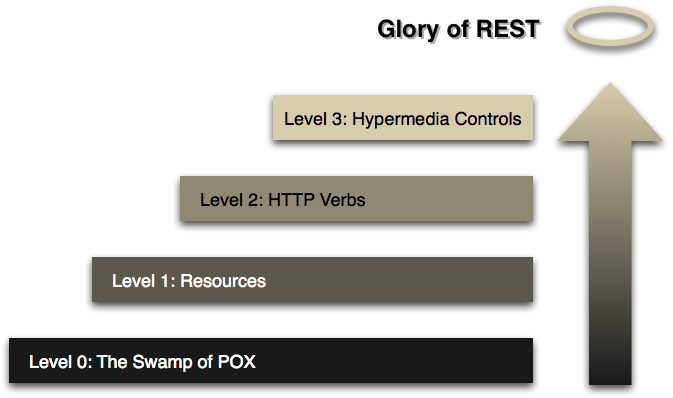
\includegraphics[width=0.8\textwidth]{rmm.png}
  \caption[Richardson Maturity Model]{Richardson Maturity Model \autocite{Fowler2010}}
  \label{fig:rmm}
\end{figure}

Een API is pas echt RESTful als het niveau 3 van het Richardson Maturity Model bereikt \autocite{Fowler2010}. HATEOAS is een belangrijk onderdeel van RESTful API design en wordt beschouwd als het hoogste niveau van volwassenheid. Echter is het implementeren van HATEOAS niet altijd eenvoudig en kan het extra complexiteit met zich meebrengen. Daarom zullen we in een volgend hoofdstuk grondig analyseren of de voordelen van HATEOAS opwegen tegen de nadelen in onze specifieke situatie.

\section{HATEOAS}

HATEOAS (Hypermedia as the Engine of Application State) is een belangrijk onderdeel van RESTful API design en vertegenwoordigt het hoogste niveau van volwassenheid volgens het Richardson Maturity Model (niveau 3) \autocite{Fowler2010}. Het kernidee achter HATEOAS is dat de server niet alleen data terugstuurt, maar ook hypermedia-links die de client informeren over welke acties mogelijk zijn op de opgevraagde data. Deze links fungeren als een soort "knoppen" in de API, die dynamisch veranderen afhankelijk van de status en rechten van de gebruiker.

\subsection{Werking van HATEOAS}

In een HATEOAS-API bevat elke response, naast de gevraagde data, ook links naar gerelateerde resources en mogelijke acties. Deze links worden meestal weergegeven in een gestandaardiseerd formaat, zoals JSON HAL (Hypertext Application Language) of Siren.

\begin{listing}[H]
  \begin{minted}{json}
  {
    "name": "Lars Salembier",
    "email": "lars.salembier@example.com",
    "_links": {
      "self": { "href": "/users/123" },
      "orders": { "href": "/users/123/orders" },
      "update": { "href": "/users/123", "method": "PUT" }
    }
  }
  \end{minted}
  \caption[Voorbeeld van een JSON HAL response]{Voorbeeld van een JSON HAL response met links naar gerelateerde resources en acties.}
  \label{lst:json_hal_example}
\end{listing}

In dit voorbeeld ziet u een JSON-object dat informatie over een gebruiker bevat. Naast de naam en het e-mailadres bevat het object ook een \texttt{links} sectie. Deze sectie bevat links naar gerelateerde resources, zoals de bestellingen van de gebruiker (\texttt{orders}), en mogelijke acties, zoals het bijwerken van de gebruikersgegevens (\texttt{update}). Elke link heeft een \texttt{href} attribuut dat de URL van de resource of actie specificeert, en optioneel een \texttt{method} attribuut dat de HTTP-methode aangeeft die gebruikt moet worden.

\subsection{Voordelen van HATEOAS}

Het gebruik van HATEOAS biedt verschillende voordelen:

\begin{itemize}
  \item \textbf{Loose Coupling:} Clients zijn minder afhankelijk van hardgecodeerde URI's. Als de serverstructuur verandert, hoeven de clients niet aangepast te worden, zolang de links correct blijven functioneren.
  \item \textbf{Ontdekkingsmogelijkheden:} Clients kunnen de API dynamisch ontdekken door de links in de responses te volgen. Dit vereenvoudigt de integratie en maakt de API meer zelfbeschrijvend.
  \item \textbf{Flexibiliteit:} De server kan de beschikbare acties en resources dynamisch aanpassen, zonder dat clients moeten worden bijgewerkt.
  \item \textbf{Documentatie:} HATEOAS kan de documentatie van de API vereenvoudigen, omdat de links zelf al informatie geven over de mogelijke acties en resources.
\end{itemize}

\subsection{Nadelen van HATEOAS}

\begin{itemize}
  \item \textbf{Complexiteit:} Het implementeren van HATEOAS kan complex zijn, vooral bij het ontwerpen van de API en het genereren van de juiste links.
  \item \textbf{Performance:} Het toevoegen van hypermedia-links aan elke response kan de performance van de API beïnvloeden, vooral bij grote datasets.
  \item \textbf{Overhead:} Het toevoegen van hypermedia-links aan elke response kan de grootte van de responses vergroten, wat kan leiden tot overhead.
  \item \textbf{Vendor Lock-in:} Het gebruik van HATEOAS kan leiden tot vendor lock-in, omdat clients afhankelijk zijn van de specifieke implementatie van de API.
  \item \textbf{Beveiliging:} Het toevoegen van hypermedia-links kan beveiligingsrisico's met zich meebrengen, zoals het blootstellen van gevoelige informatie.
  \item \textbf{Caching:} Het cachen van responses kan moeilijker zijn, omdat de links dynamisch gegenereerd worden.
\end{itemize}

\section{OpenAPI}

OpenAPI (voorheen bekend als Swagger) is een specificatie voor het beschrijven van RESTful API's in een machine-leesbaar formaat, meestal YAML of JSON \autocite{OpenAPIInitiative2021}. Het biedt een gestandaardiseerde manier om de structuur en functionaliteit van een API te documenteren, inclusief endpoints, parameters, request bodies, response bodies, authenticatiemethoden en meer. Deze documentatie kan vervolgens gebruikt worden voor diverse doeleinden, zoals het genereren van interactieve API documentatie, het automatisch genereren van client- en servercode, en het testen van de API.

\subsection{Structuur van een OpenAPI document}

Een OpenAPI document bevat verschillende secties die de API beschrijven:

\begin{itemize}
    \item \textbf{openapi:} De OpenAPI specificatie versie.
    \item \textbf{info:} Metadata over de API, zoals de titel, beschrijving en versie.
    \item \textbf{servers:} Een lijst van servers waar de API beschikbaar is.
    \item \textbf{paths:} De endpoints van de API, inclusief de ondersteunde HTTP-methoden en parameters.
    \item \textbf{components:} Herbruikbare componenten, zoals schemas (datatypes) en security schemes.
    \item \textbf{security:} De beveiligingsmechanismen die gebruikt worden door de API.
    \item \textbf{tags:} Tags om de API te categoriseren.
    \item \textbf{externalDocs:} Links naar externe documentatie.
\end{itemize}

\begin{listing}[H]
\begin{minted}{yaml}
openapi: 3.0.0
info:
  title: BrightEats API
  version: v1
paths:
  /orders:
    get:
      summary: Haal alle bestellingen op
      responses:
        '200':
          description: Lijst met bestellingen
          content:
            application/json:
              schema:
                type: array
                items:
                  $ref: '#/components/schemas/Order'
components:
  schemas:
    Order:
      type: object
      properties:
        id:
          type: integer
        description:
          type: string
\end{minted}
\caption[Voorbeeld van een OpenAPI document in YAML]{Voorbeeld van een OpenAPI document in YAML dat een endpoint beschrijft om bestellingen op te halen.}
\label{lst:openapi_example}
\end{listing}


\subsection{Tools voor OpenAPI}

Er zijn verschillende tools beschikbaar die werken met OpenAPI-documenten:

\begin{itemize}
  \item \textbf{Swagger UI:} Genereert interactieve documentatie waarmee gebruikers de API kunnen verkennen en testen.
  \item \textbf{Redoc:} Genereert statische documentatie in een aantrekkelijke en leesbare vorm.
  \item \textbf{OpenAPI Generator:} Genereert client- en servercode in verschillende programmeertalen op basis van een OpenAPI document.
  \item \textbf{Postman:} Ondersteunt het importeren en exporteren van OpenAPI-documenten en kan gebruikt worden voor het testen van de API.
\end{itemize}

\subsection{Voordelen van OpenAPI}

\begin{itemize}
  \item \textbf{Gestandaardiseerde documentatie:} OpenAPI biedt een gestandaardiseerde manier om API's te documenteren, waardoor de documentatie consistent en gemakkelijk te begrijpen is.
  \item \textbf{Automatische documentatiegeneratie:} Tools zoals Swagger UI en Redoc kunnen automatisch documentatie genereren op basis van een OpenAPI-document, waardoor de documentatie altijd up-to-date is.
  \item \textbf{Codegeneratie:} OpenAPI Generator kan client- en servercode genereren in verschillende programmeertalen, waardoor ontwikkeltijd wordt bespaard.
  \item \textbf{Testen:} OpenAPI-documenten kunnen gebruikt worden voor het automatisch testen van de API.
  \item \textbf{Samenwerking:} OpenAPI vergemakkelijkt de samenwerking tussen frontend- en backend-teams door een duidelijke en gedeelde specificatie van de API te bieden.
\end{itemize}

\subsection{Nadelen van OpenAPI}

\begin{itemize}
  \item \textbf{Leercurve:} Het leren schrijven en onderhouden van OpenAPI-documenten vereist enige inspanning.
  \item \textbf{Onderhoud:} OpenAPI documenten moeten up-to-date gehouden worden met de API, wat extra onderhoud vereist. Dit kan echter ook als een voordeel worden beschouwd, omdat het dwingt tot het consistent documenteren van de API.
\end{itemize}

\section{HATEOAS: Een evaluatie voor BrightAnalytics}

HATEOAS (Hypermedia as the Engine of Application State) vertegenwoordigt het hoogste niveau van volwassenheid binnen RESTful API design volgens het Richardson Maturity Model (niveau 3) \autocite{Fowler2010}. In dit hoofdstuk evalueren we de toepasbaarheid van HATEOAS binnen de specifieke context van BrightAnalytics. Hoewel HATEOAS theoretisch voordelen biedt, zullen we aantonen dat de implementatie ervan in onze situatie niet gerechtvaardigd is.

\subsection{Baten}

HATEOAS beidt clients de mogelijkheid om een API dynamisch te ontdekken en te navigeren zonder voorafgaande kennis van de URI-structuur. Elke response bevat hypermedia-links die de client informeren over de beschikbare acties en gerelateerde resources. Dit biedt potentiële voordelen zoals:

\begin{itemize}
  \item \textbf{Loose Coupling:} Clients zijn minder afhankelijk van hardgecodeerde URI's, waardoor de serverstructuur kan evolueren zonder directe impact op de clients.
  \item \textbf{Ontdekkingsmogelijkheden:} Clients kunnen de API dynamisch verkennen door de aangeboden links te volgen.
  \item \textbf{Flexibiliteit:} De server kan de beschikbare acties en resources dynamisch aanpassen.
\end{itemize}

\subsection{Kosten}

Een cruciaal aspect van onze situatie is dat de te ontwikkelen API's uitsluitend intern gebruikt zullen worden binnen BrightAnalytics. Dit betekent dat de development teams directe toegang hebben tot uitgebreide documentatie en effectief kunnen communiceren over de API-structuur. De noodzaak voor de ontdekkingsmogelijkheden die HATEOAS biedt, wordt hierdoor sterk gereduceerd.

\bigskip

De implementatie van HATEOAS brengt aanzienlijke kosten met zich mee, die in onze context niet opwegen tegen de beperkte voordelen.

\bigskip

Het genereren en beheren van hypermedia-links introduceert extra complexiteit in de ontwikkeling van de API. Dit vereist een doordachte implementatie en grondig testen om de correctheid en consistentie van de links te garanderen.

\bigskip

Het toevoegen van hypermedia-links aan elke response vergroot de hoeveelheid data die verzonden moet worden. Dit kan een negatieve impact hebben op de performance, met name bij grote datasets.

\bigskip

Gezien de interne context en de reeds aanwezige communicatiekanalen binnen de development teams, is de meerwaarde van HATEOAS beperkt. De kosten van implementatie en onderhoud wegen niet op tegen de minimale winst in ontdekkingsmogelijkheden.

\bigskip

De ontwikkeling van de API's zal gepaard gaan met uitgebreide documentatie gebaseerd op de OpenAPI specificatie. Met behulp van tools zoals Swagger UI of Redoc zal deze documentatie interactief en gemakkelijk toegankelijk zijn voor alle betrokken developers. Dit biedt een effectief alternatief voor de ontdekkingsmogelijkheden van HATEOAS, zonder de bijbehorende complexiteit en overhead.

\subsection{Conclusie}

Gezien de interne context van de API's bij BrightAnalytics en de beschikbaarheid van uitgebreide OpenAPI documentatie, concluderen we dat de implementatie van HATEOAS niet gerechtvaardigd is. De kosten en complexiteit wegen niet op tegen de beperkte voordelen. Daarom kiezen we ervoor om HATEOAS niet te implementeren in onze API's.

\section{RESTful API best practices en de Zalando Guidelines}

Het ontwerpen en implementeren van hoogwaardige, onderhoudbare en schaalbare RESTful API's vereist het volgen van best practices. Hoewel een gedetailleerde bespreking van alle best practices buiten het bestek van deze literatuurstudie valt, erkennen we het belang ervan en zullen we een set specifieke richtlijnen opstellen tijdens de ontwikkelingsfase van onze API's. Hierbij zullen we ons baseren op de uitgebreide \textit{Zalando RESTful API Guidelines} \autocite{ZAG2024}.

\subsection{De Zalando RESTful API Guidelines}

De Zalando RESTful API Guidelines bieden een uitgebreid framework voor het ontwerpen en ontwikkelen van RESTful API's. Deze guidelines behandelen een breed scala aan onderwerpen, waaronder:

\begin{itemize}
  \item \textbf{URI Design:} Richtlijnen voor het creëren van consistente, leesbare en betekenisvolle URI's.
  \item \textbf{HTTP Methoden:} Correct gebruik van HTTP methoden (GET, POST, PUT, PATCH, DELETE) en hun semantische betekenis.
  \item \textbf{Status Codes:} Gebruik van de juiste HTTP status codes om de uitkomst van requests te communiceren.
  \item \textbf{Dataformaten:} Richtlijnen voor het gebruik van de juiste dataformaten.
  \item \textbf{Versionering:} Strategieën voor het beheren van API versies en het waarborgen van backward compatibility.
  \item \textbf{Foutbehandeling:} Best practices voor het afhandelen en rapporteren van fouten.
  \item \textbf{Authenticatie en Autorisatie:} Beveiligingsmechanismen voor het beschermen van de API.
  \item \textbf{Documentatie:} Het belang van duidelijke en complete API documentatie.
  \item \textbf{Paginering:} Technieken voor het efficiënt verwerken van grote datasets.
  \item \textbf{Filtering en Sortering:} Mogelijkheden voor clients om data te filteren en te sorteren.
\end{itemize}

De Zalando RESTful API Guidelines bieden een waardevolle bron van best practices en richtlijnen voor het ontwerpen van RESTful API's. We zullen deze guidelines gebruiken als basis voor het opstellen van onze eigen set richtlijnen tijdens de ontwikkeling van de BrightEats API.

\section{Implementatie met Laravel en Vue.js}

Dit hoofdstuk beschrijft de gekozen technologieën voor de backend en frontend ontwikkeling, namelijk Laravel en Vue.js, en hoe de concepten van RESTful API design en OpenAPI daarop worden toegepast.

\subsection{Laravel als backend framework}

Laravel is een populair PHP framework dat zich uitstekend leent voor het ontwikkelen van robuuste en schaalbare webapplicaties, inclusief RESTful API's. We kiezen voor Laravel vanwege de volgende redenen \autocite{Laravel}:

\begin{itemize}
  \item \textbf{MVC Architectuur:} Laravel's Model-View-Controller architectuur bevordert een gestructureerde en modulaire codebase, wat de ontwikkeling en onderhoudbaarheid van API's vereenvoudigt.
  \item \textbf{Eloquent ORM:} De Eloquent ORM (Object-Relational Mapper) maakt het eenvoudig om te interageren met databases en data te manipuleren.
  \item \textbf{Routing:} Laravel biedt een flexibel en krachtig routing systeem voor het definiëren van API endpoints.
  \item \textbf{Middleware:} Middleware in Laravel kan gebruikt worden voor taken zoals authenticatie, autorisatie, logging en request validatie.
  \item \textbf{Testing:} Laravel biedt uitgebreide mogelijkheden voor het testen van API's.
  \item \textbf{Community en Documentatie:} Laravel heeft een grote en actieve community en uitgebreide documentatie, wat de ontwikkeling vergemakkelijkt.
\end{itemize}

\subsubsection{RESTful API's in Laravel}

Laravel biedt ingebouwde ondersteuning voor het ontwikkelen van RESTful API's. Resources kunnen worden gedefinieerd met behulp van resource controllers en routes.

\begin{listing}[H]
\begin{minted}{php}
  use App\Models\Product;
  use Illuminate\Http\Request;
  use App\Http\Resources\ProductResource;
  
  class ProductController extends Controller
  {
    public function index()
    {
      return ProductResource::collection(Product::all());
    }

    public function show(Product $product)
    {
      return new ProductResource($product);
    }

    public function store(Request $request)
    {
      $validated = $request->validate([
        'name' => 'required|max:255',
        'price' => 'required|numeric',
      ]);

      $product = Product::create($validated);

      return new ProductResource($product);
    }

    // ... update, destroy methods ...
  }
\end{minted}
\caption[Voorbeeld van een Laravel resource controller]{Voorbeeld van een Laravel resource controller voor het beheren van producten.}
\label{lst:laravel_controller}
\end{listing}

\subsection{Vue.js als frontend framework}

Vue.js is een progressief JavaScript framework dat ideaal is voor het bouwen van interactieve user interfaces \autocite{VueJS}. We kiezen voor Vue.js vanwege:

\begin{itemize}
  \item \textbf{Component-gebaseerde architectuur:} Vue.js stimuleert het ontwikkelen van herbruikbare componenten, wat de codebase overzichtelijker en onderhoudbaarder maakt.
  \item \textbf{Reactiviteit:} Vue.js' reactieve data binding zorgt ervoor dat de user interface automatisch wordt bijgewerkt wanneer de data verandert.
  \item \textbf{Eenvoudige integratie:} Vue.js kan gemakkelijk geïntegreerd worden met andere libraries en frameworks.
  \item \textbf{Performance:} Vue.js is lightweight en performant.
  \item \textbf{Community en Documentatie:} Net als Laravel heeft Vue.js een grote en actieve community en uitgebreide documentatie.
\end{itemize}

\subsubsection{Consumptie van de API in Vue.js}

Vue.js-applicaties kunnen de Laravel API consumeren met behulp van HTTP clients zoals Axios of de ingebouwde Fetch API. Data opgehaald van de API kan vervolgens gebruikt worden om de user interface dynamisch te vullen.

\begin{listing}[H]
\begin{minted}{javascript}
  <template>
  <ul>
    <li v-for="product in products" :key="product.id">
      {{ product.name }} - {{ product.price }}
    </li>
  </ul>
  </template>

  <script>
  import axios from 'axios';

  export default {
  data() {
    return {
      products: [],
    };
  },
  mounted() {
    axios.get('/api/products')
      .then(response => {
        this.products = response.data.data;
      })
      .catch(error => {
        console.error(error);
      });
  },
  };
  </script>
\end{minted}
\caption[Voorbeeld van het ophalen van data van een Laravel API in Vue.js]{Voorbeeld van het ophalen van data van een Laravel API in Vue.js met behulp van Axios.}
\label{lst:vue_axios}
\end{listing}

\subsection{OpenAPI integratie}

OpenAPI zal een centrale rol spelen in de ontwikkeling van onze API's. We zullen een OpenAPI-document creëren dat de API volledig beschrijft. Dit document zal dienen als basis voor:

\begin{itemize}
  \item \textbf{Documentatie:} Automatische generatie van interactieve documentatie met behulp van tools zoals Swagger UI.
  \item \textbf{Client code generatie:} Mogelijkheid om client code te genereren in verschillende talen.
  \item \textbf{Server side validatie:} Validatie van requests en responses op basis van het OpenAPI schema.
  \item \textbf{Testing:} Automatische tests genereren op basis van het OpenAPI document.
\end{itemize}

Door OpenAPI te integreren in ons ontwikkelproces, zorgen we voor een consistente, goed gedocumenteerde en gemakkelijk te onderhouden API.

\begin{listing}[H]
\begin{minted}{yaml}
paths:
  /products:
    get:
      summary: Get all products
      responses:
        '200':
          description: A list of products
          content:
            application/json:
              schema:
                type: object
                properties:
                  data:
                    type: array
                    items:
                      $ref: '#/components/schemas/Product'
components:
  schemas:
    Product:
      type: object
      properties:
        id:
          type: integer
          readOnly: true
        name:
          type: string
        price:
          type: number
          format: float
\end{minted}
\caption[Voorbeeld van een OpenAPI document in YAML]{Voorbeeld van een OpenAPI document in YAML dat een endpoint beschrijft om producten op te halen.}
\label{lst:openapi_example_resource}
\end{listing}

\section{Conclusie}

Deze literatuurstudie heeft een overzicht geboden van de belangrijkste concepten en technologieën die relevant zijn voor het ontwikkelen van robuuste, schaalbare en goed gedocumenteerde RESTful API's, met specifieke aandacht voor de context van BrightAnalytics en hun bestaande technologie stack. We begonnen met een inleiding tot API's in het algemeen, waarna we de principes van RESTful API design hebben geanalyseerd, inclusief de zes belangrijkste principes (Client-Server, Stateless, Cacheable, Uniform Interface, Layered System en Code-On-Demand), HTTP methoden, status codes en het resource-gebaseerde karakter van REST.

\bigskip

Vervolgens introduceerden we het Richardson Maturity Model, dat de volwassenheid van RESTful API's beschrijft, met speciale aandacht voor HATEOAS. Na een grondige evaluatie van de voor- en nadelen van HATEOAS, in combinatie met de specifieke context van BrightAnalytics - interne API's en een nadruk op heldere documentatie - concludeerden we dat de implementatie van HATEOAS voor dit project niet de meest efficiënte aanpak is. De complexiteit en overhead wegen niet op tegen de beperkte voordelen in onze situatie. Deze beslissing wordt versterkt door onze keuze voor OpenAPI, waarmee we uitgebreide en interactieve documentatie zullen genereren, wat de noodzaak voor de ontdekkingsaspecten van HATEOAS minimaliseert.

\bigskip

OpenAPI vormt een kerncomponent in onze API-ontwikkelingsstrategie. Door een OpenAPI-document te creëren dat de API volledig beschrijft, waarborgen we consistente documentatie, automatische codegeneratie, server-side validatie en geautomatiseerd testen. Dit bevordert de kwaliteit, onderhoudbaarheid en schaalbaarheid van onze API's. De integratie van OpenAPI, gecombineerd met de techstack van BrightAnalytics (Laravel en Vue.js), optimaliseert ons ontwikkelproces.

\bigskip

Ten slotte benadrukten we het belang van best practices voor API-ontwikkeling. Een gedetailleerde beschrijving hiervan valt buiten het bestek van deze literatuurstudie, maar tijdens de ontwikkeling zullen we specifieke richtlijnen formuleren, gebaseerd op de Zalando RESTful API Guidelines. Dit framework biedt een solide basis voor het ontwerpen en implementeren van RESTful API's, waarmee we de consistentie, betrouwbaarheid en schaalbaarheid van onze API's willen verhogen.

%%=============================================================================
%% Methodologie
%%=============================================================================

\chapter{\IfLanguageName{dutch}{Methodologie}{Methodology}}%
\label{ch:methodologie}

Deze bachelorproef onderzoekt en verbetert de API-kwaliteit bij BrightAnalytics door de iteratieve ontwikkeling van de BrightEats API. Onderzoek en ontwikkeling gaan hand in hand. De inzichten uit het onderzoek worden direct toegepast op de API, en de ervaringen tijdens de ontwikkeling sturen het onderzoek bij.

Ik ga ervan uit dat ik elke week minstens \'e\'en dag kan werken aan de bachelorproef. De deadlines zijn echter flexibel, aangezien de API-ontwikkeling continu doorloopt en de planning kan be\"invloeden.

Na evaluatie in de literatuurstudie blijkt implementatie van HATEOAS niet geschikt voor de BrightEats API. In plaats daarvan focussen we op het opstellen van een interne guide, gebaseerd op best practices en vergelijkbaar met de Zalando RESTful API and Event Scheme Guidelines. Daarnaast wordt een uitgebreide OpenAPI-specificatie voor de API ontwikkeld.

\section{Fase 1: Onderzoek en eerste opzet API}

\textbf{Deadline: 17 november 2024}

Deze fase is gericht op het verzamelen van kennis over kwalitatieve API-ontwikkeling en het defini\"eren van een eerste set best practices voor BrightEats. Ik bestudeer de principes van REST, HATEOAS en OpenAPI en hun belang voor API-kwaliteit en formuleer concrete aanbevelingen voor de BrightEats API.

\bigskip

\textbf{We zoeken een antwoord op de volgende vragen:}
\begin{itemize}
  \item Wat zijn de principes van REST?
  \item Hoe dragen deze bij aan betere API's?
  \item Welke best practices zijn er voor URI-structuur, HTTP-methoden, response codes en versiebeheer?
  \item Hoe houden we onze Laravel-API RESTful?
  \item Wat zijn de principes en voordelen van HATEOAS?
  \item Hoe kunnen we HATEOAS implementeren in een Laravel-API?
  \item Hoe maken we optimaal gebruik van HATEOAS in de frontend van BrightEats?
  \item Wat is OpenAPI en hoe kan dit worden toegepast in de documentatie van een Laravel-API?
\end{itemize}

\textbf{Deliverables:}

\begin{itemize}
  \item Literatuurstudie over REST, HATEOAS en OpenAPI.
  \item Best practices voor de implementatie in de BrightEats API en frontend.
\end{itemize}

\section{Fase 2: Iteratieve ontwikkeling en verfijning BrightEats API}

\textbf{Deadline: 8 december 2024}

\bigskip
Gedurende deze fase refactor ik de BrightEats API iteratief naar een RESTful design, terwijl we ook de OpenAPI-specificatie definiëren. We doen dit stap per stap, zonder de hele API in één keer te herschrijven. De focus ligt op het toepassen van de best practices die we in fase 1 hebben geformuleerd.

\subsection{Ontwikkeling van de API (doorlopend)}

\bigskip
Elke week doorloop ik de volgende stappen:

\begin{enumerate}
  \item \textbf{Plannen:} Ik bepaal welke functionaliteiten ik aan de API zal toevoegen (of welke code ik ga refactoren om zo aan de nieuwe best practices te voldoen)
  \item \textbf{Ontwerpen:} Ik ontwerp de nieuwe/gerefactorde functionaliteiten met de best practices in gedachten.
  \item \textbf{Implementeren:} Ik programeer de nieuwe/gerefactorde functionaliteiten in de API.
  \item \textbf{Testen:} Ik test de nieuwe/gerefactorde functionaliteiten grondig.
  \item \textbf{Evalueren:} Ik beoordeel de kwaliteit, structuur en gebruikte best practices.
  \item \textbf{Best practices bijstellen:} Ik pas de richtlijnen aan op basis van de evaluatie en feedback.
\end{enumerate}

\textbf{Deliverables:}

\begin{itemize}
  \item Een concrete set best practices voor de BrightEats API.
  \item De API zelf, volgens de best practices.
\end{itemize}

\section{Fase 3: Synthese, aanbevelingen en afronding}

\textbf{Deadline: 15 december 2025}

\bigskip
In de laatste fase vat ik mijn bevindingen samen en formuleer ik een antwoord op de onderzoeksvraag. Wat was de exacte kost van het implementeren van OpenAPI en RESTfulness in de BrightEats API? Welke voordelen en nadelen bracht dit met zich mee? Welke best practices kunnen we formuleren voor de ontwikkeling van API's bij BrightAnalytics?

\subsection{Synthese \& Aanbevelingen}

\textbf{Deadline: 15 januari 2025}

\bigskip
Ik schrijf de conclusie en aanbevelingen voor BrightAnalytics. Hierbij beantwoord ik de deelvragen en onderzoeksvraag en formuleer ik concrete best practices voor de ontwikkeling van RESTful API's bij BrightAnalytics.

\subsection{Afronding bachelorproef}

\textbf{Deadline: 10 januari 2025}

\bigskip
Ik werk de bachelorproef af, rekening houdend met de feedback van de promotor en de copromotor bij BrightAnalytics.

\textbf{Deliverables:}

\begin{itemize}
  \item Concrete aanbevelingen voor beter API-ontwerp.
  \item Finale versie van de bachelorproef.
\end{itemize}

\section{Gantt chart}

\begin{figure}[H]
  \centering
  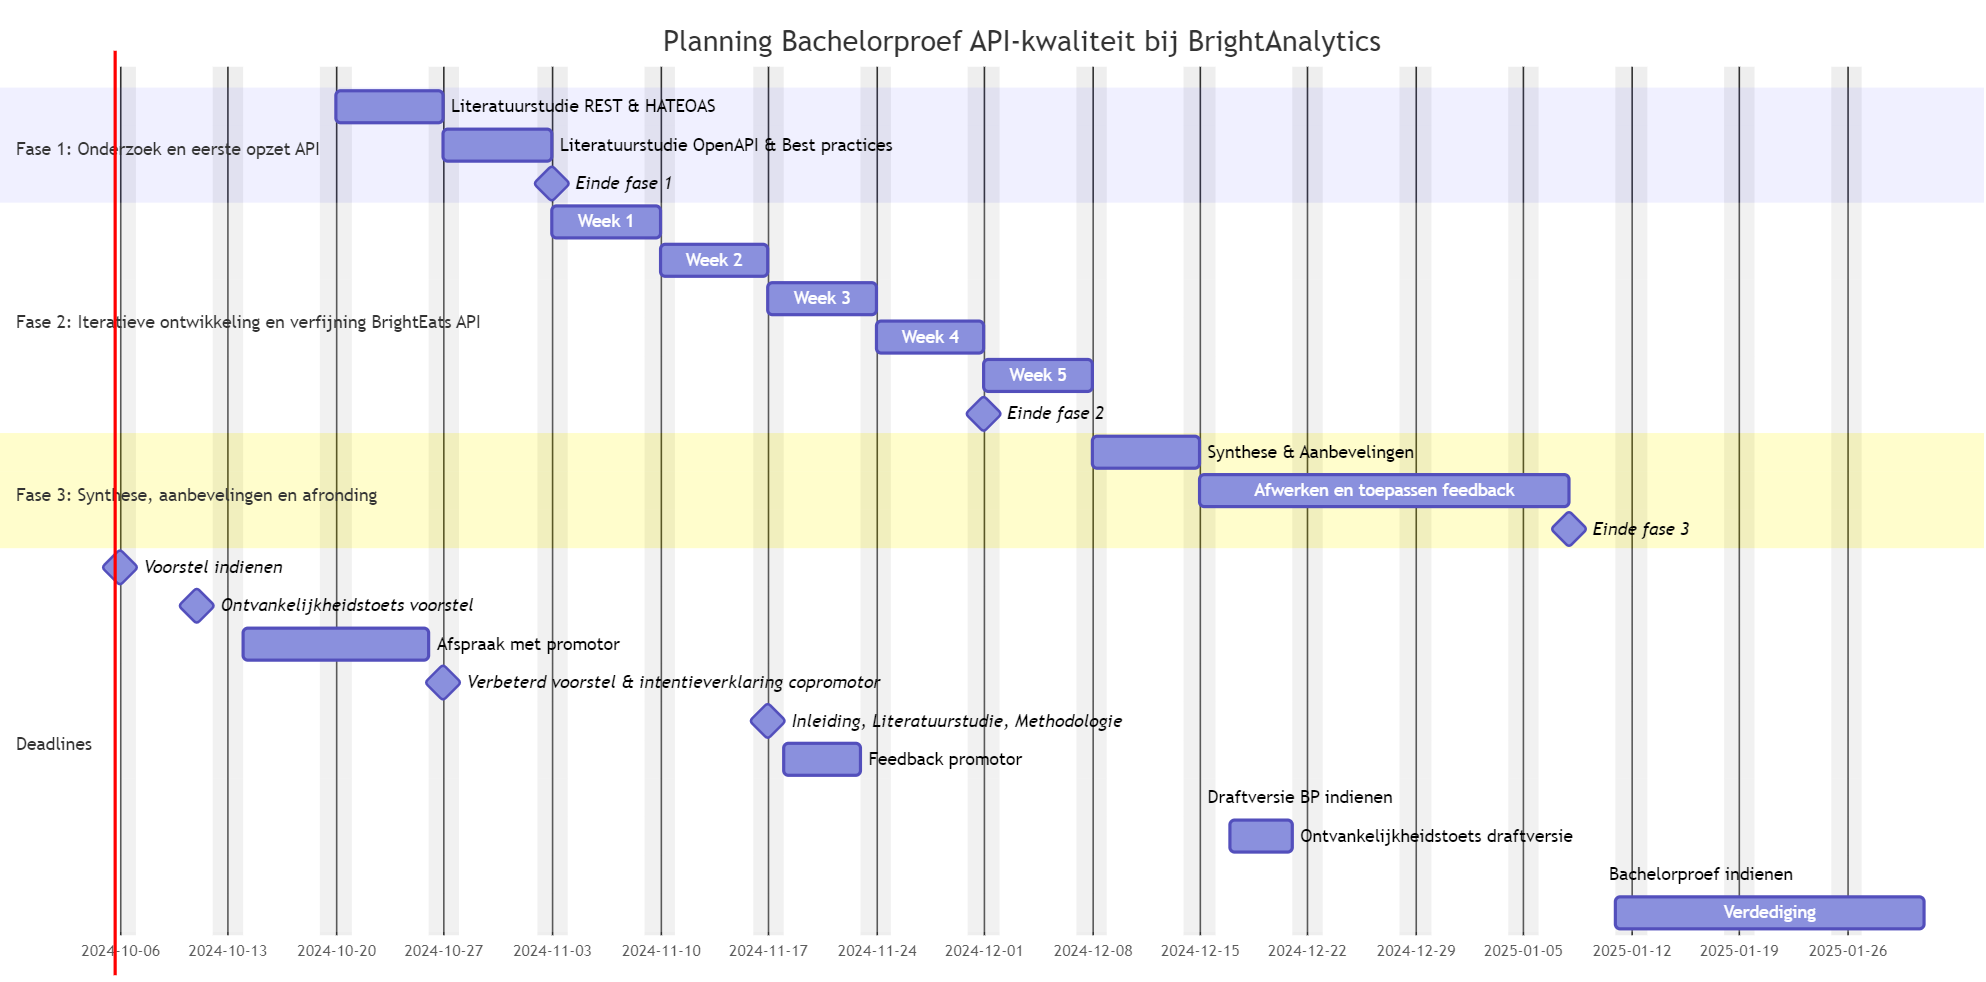
\includegraphics[width=0.8\textwidth]{gantt.png}
  \caption{Gantt chart van de methodologie}
  \label{fig:gantt}
\end{figure}


% Voeg hier je eigen hoofdstukken toe die de ``corpus'' van je bachelorproef
% vormen. De structuur en titels hangen af van je eigen onderzoek. Je kan bv.
% elke fase in je onderzoek in een apart hoofdstuk bespreken.

%\input{...}
%\input{...}
%...

%%=============================================================================
%% Conclusie
%%=============================================================================

\chapter{Conclusie}%
\label{ch:conclusie}

Dit hoofdstuk sluit deze bachelorproef af door de belangrijkste bevindingen samen te vatten en de centrale onderzoeksvraag te beantwoorden. Op basis van de resultaten en evaluatie uit het vorige hoofdstuk formuleren we concrete aanbevelingen voor de ontwikkeling van RESTful API's bij BrightAnalytics, met focus op het verbeteren van kwaliteit, consistentie en onderhoudbaarheid.

\bigskip

De implementatie van RESTful API principes en de OpenAPI specificatie in de Bright\-Eats API heeft geleid tot significante verbeteringen op verschillende vlakken:

\begin{itemize}
  \item \textbf{Kwaliteit:} De kwaliteit van de API is aanzienlijk verbeterd door de implementatie van geautomatiseerde tests en een focus op robuustheid. De API is stabieler, betrouwbaarder en beter bestand tegen fouten.
  \item \textbf{Consistentie:} De API is consistent in design en implementatie dankzij de strikte naleving van RESTful principes en het gebruik van onze opgestelde guidelines. De endpoints zijn uniform ontworpen, HTTP response codes worden correct gebruikt en datastructuren zijn voorspelbaar. Er is nog ruimte voor verbetering in de responses zelf.
  \item \textbf{Onderhoudbaarheid:} De onderhoudbaarheid van de API is sterk verbeterd door de gestructureerde code, de uitgebreide documentatie en de test suite. De tijd besteed aan debugging is verminderd en het toevoegen van nieuwe features is eenvoudiger geworden.
\end{itemize}

De implementatie van de OpenAPI specificatie was de grootste kostenpost, met name de tijd die nodig was om PHPDoc comments toe te voegen aan de code. Deze initiële investering heeft zich echter terugbetaald in de vorm van automatisch gegenereerde documentatie, verbeterde communicatie, eenvoudigere debugging en snellere onboarding van nieuwe developers.

\bigskip

De evaluatie van de Bright\-Eats API toont aan dat de implementatie van RESTful API principes en de OpenAPI specificatie een positieve impact heeft op de kwaliteit, consistentie en onderhoudbaarheid van de API. De API is stabieler, betrouwbaarder en beter bestand tegen fouten. De endpoints zijn uniform ontworpen, HTTP response codes worden correct gebruikt en datastructuren zijn voorspelbaar. De onderhoudbaarheid van de API is sterk verbeterd door de gestructureerde code, de uitgebreide documentatie en de test suite.

\section{Antwoord op de onderzoeksvraag}

De centrale onderzoeksvraag van deze bachelorproef luidt als volgt:

\begin{displayquote}
  \textit{Welke concrete voordelen biedt de implementatie van RESTful API design, en in het bijzonder HATEOAS en OpenAPI, voor de kwaliteit, consistentie en onderhoudbaarheid van een Laravel-API en een bijbehorende frontend applicatie?}
\end{displayquote}

Op basis van de bevindingen uit dit onderzoek kunnen we deze vraag als volgt beantwoorden:

\subsection{RESTful API design}

De implementatie van RESTful API design principes heeft een positieve impact gehad op de kwaliteit, consistentie en onderhoudbaarheid van de Bright\-Eats Laravel-API. De gestructureerde aanpak, met een duidelijke scheiding van concerns (controllers, services, models), een consistent gebruik van HTTP methoden en status codes, en de toepassing en opstelling van een set duidelijke guidelines, heeft geresulteerd in een robuuste, voorspelbare en makkelijk te begrijpen API. Dit heeft op zijn beurt geleid tot een verhoogde kwaliteit van de code, een snellere ontwikkeling en een verbeterde onderhoudbaarheid.

\subsection{HATEOAS}

De beslissing om HATEOAS \textit{niet} te implementeren bleek de juiste te zijn. De meerwaarde van HATEOAS in het geval van de Bright\-Eats API, die enkel intern bij BrightAnalytics gebruikt wordt, woog niet op tegen de complexiteit en overhead die gepaard gaan met de implementatie ervan. De uitgebreide documentatie gegenereerd door OpenAPI, in combinatie met de duidelijke communicatie binnen het development team, biedt voldoende mogelijkheden voor ontwikkelaars om de API te begrijpen en te gebruiken.

\subsection{OpenAPI}

OpenAPI heeft een cruciale rol gespeeld in het verbeteren van de documentatie en standaardisatie van de API. De automatisch gegenereerde, interactieve documentatie dient als een centrale bron van waarheid voor alle ontwikkelaars en vereenvoudigt de samenwerking tussen frontend en backend teams. Bovendien opent OpenAPI de mogelijkheid voor toekomstige automatisering, zoals het genereren van client SDK's en het valideren van requests en responses.

\section{Aanbevelingen}

De aanbevelingen voor API design bij BrightAnalytics zijn opgesteld in hoofdstuk 4 van deze bachelorproef. Hier gaan we concreet bepalen wat een RESTful API is en zorgen we voor minder ambigu\"iteit in API responses, requests, query parameters, foutafhandeling, caching en versiebeheer. Dit document dient een startpunt te worden voor een goede set guidelines die in het algemeen kunnen worden gebruikt voor het bouwen van performante, robuuste en onderhoudbare API's.

\bigskip

Niet alle guidelines die werden opgesteld in dit onderzoek zijn even relevant voor elk project. Voor Bright\-Eats bijvoorbeeld hebben we de meer geavanceerde guidelines over query parameters, filters en sortering niet moeten implementeren. Voor andere projecten zullen andere delen van de guidelines minder of meer relevant zijn. Het is belangrijk om de guidelines te zien als een set van best practices die kunnen worden aangepast aan de specifieke noden van elk project.

\bigskip

Daarnaast raden we aan om de implementatie van OpenAPI verder te onderzoeken en te integreren in de bestaande ontwikkelprocessen. De voordelen van automatisch gegenereerde documentatie, standaardisatie en automatisering wegen op tegen de initi\"ele investering die nodig is om de specificatie op te stellen. Het is belangrijk om de documentatie up-to-date te houden en te integreren in de dagelijkse workflow van de ontwikkelaars. Op die manier wordt de documentatie een levend document dat een centrale bron van waarheid vormt voor alle betrokken partijen.

\section{Reflectie en toekomstig onderzoek}

Het onderzoeksproces verliep over het algemeen vlot. De iteratieve aanpak, waarbij de API stapsgewijs werd ontwikkeld en getest, bleek effectief. De keuze om vroeg in het proces te focussen op OpenAPI heeft de documentatie en consistentie van de API sterk verbeterd.

\bigskip

Een punt van verbetering is de diepgang van de evaluatie van de onderhoudskosten. Hoewel de tijd besteed aan debugging is afgenomen naarmate de API meer RESTful werd, is het lastig om dit exact te kwantificeren. Een meer gedetailleerde tracking van de ontwikkeltijd had hier meer inzicht in kunnen geven.

\bigskip

Een beperking van dit onderzoek is de focus op een specifieke use case, namelijk de Bright\-Eats API. De bevindingen zijn mogelijk niet generaliseerbaar naar andere API's of andere contexten.

\subsection{Suggesties voor toekomstig onderzoek}

\begin{itemize}
  \item \textbf{Langetermijnevaluatie:} Een evaluatie van de impact van RESTful API design en OpenAPI op de onderhoudskosten op langere termijn zou waardevolle inzichten kunnen opleveren.
  \item \textbf{Vergelijking met andere API-stijlen:} Een vergelijking van de RESTful aanpak met andere API stijlen, zoals GraphQL, zou interessant zijn om de voor- en nadelen van elke stijl beter te begrijpen.
  \item \textbf{Automatische validatie met OpenAPI:} Verder onderzoek naar het gebruik van OpenAPI voor het automatisch valideren van requests en responses zou de robuustheid van API's kunnen verhogen.
  \item \textbf{API-beveiliging:} Een diepere analyse van de implementatie van API security maatregelen zou een belangrijke toevoeging zijn aan toekomstig onderzoek.
  \item \textbf{Performance testen:} Onderzoek naar de performance implicaties van verschillende API design keuzes zou waardevol zijn voor het optimaliseren van de API performance.
\end{itemize}

\section{Afsluiting}

Goed API-ontwerp is essentieel voor het succes van moderne software applicaties. Een goed ontworpen API is niet alleen robuust, consistent en onderhoudbaar, maar ook makkelijk te gebruiken en te integreren met andere systemen. Deze bachelorproef heeft aangetoond dat de implementatie van RESTful API principes en de OpenAPI specificatie een significante bijdrage levert aan het bereiken van deze doelen. De aanbevelingen in deze bachelorproef bieden BrightAnalytics concrete handvatten voor het ontwikkelen van hoogwaardige API's, wat de efficiëntie van het development team verhoogt en de kwaliteit van de software verbetert.


%---------- Bijlagen -----------------------------------------------------------

\appendix

\chapter{Onderzoeksvoorstel}

Het onderwerp van deze bachelorproef is gebaseerd op een onderzoeksvoorstel dat vooraf werd beoordeeld door de promotor. Dat voorstel is opgenomen in deze bijlage.

%% TODO: 
%\section*{Samenvatting}

% Kopieer en plak hier de samenvatting (abstract) van je onderzoeksvoorstel.

% Verwijzing naar het bestand met de inhoud van het onderzoeksvoorstel
%---------- Inleiding ---------------------------------------------------------

\section{Inleiding}%
\label{sec:inleiding}
De explosieve groei van data en de toenemende vraag naar naadloze integraties tussen applicaties hebben de rol van Application Programming Interfaces (API's) centraal geplaatst in de hedendaagse softwareontwikkeling. Een goed ontworpen en gedocumenteerde API is niet langer een luxe, maar essentieel voor succes in het digitale landschap. Dit is met name relevant voor BrightAnalytics, een bedrijf dat een geavanceerd data-visualisatieplatform aanbiedt voor financiële rapportering en business intelligence. De kwaliteit, consistentie en efficiëntie van de API's die BrightAnalytics ontwikkelt, zijn van cruciaal belang voor de functionaliteit van hun producten, de integratie met andere systemen en het snel kunnen ontwikkelen van nieuwe features.

\bigskip

Tijdens mijn stage bij BrightAnalytics ontwikkel ik "BrightEats", een applicatie waarmee werknemers hun lunch kunnen bestellen. Deze applicatie is afhankelijk van een backend API, geschreven in Laravel, net zoals alle andere applicaties bij BrightAnalytics. De ontwikkeling van deze API biedt een uitgelezen kans om de principes van RESTful API design te implementeren en om te evalueren welke voor- en nadelen de meer geavanceerde principes hiervan (met name OpenAPI en Hypermedia As The Engine Of Application State (HATEOAS) ) met zich meebrengen.

\bigskip

Het principe van RESTful API design werd in 2000 geïntroduceerd door Roy Fielding in zijn proefschrift \autocite{Fielding2000}. REST (Representational State Transfer) is ondertussen wijdverspreid en wordt goed ondersteund wanneer we een API willen bouwen met Laravel. Echter zijn de meer geavanceerde onderdelen van REST, met name HATEOAS (Hypermedia As The Engine Of Application State) en OpenAPI, minder bekend en worden ze minder vaak toegepast in de praktijk. Deze principes kunnen echter een grote impact hebben op de kwaliteit, consistentie en onderhoudbaarheid van een API.

\bigskip

Met deze bachelorproef proberen we een antwoord te formuleren op de volgende onderzoeksvraag:

\begin{center}
\textbf{Welke concrete voordelen biedt de implementatie van RESTful API design, en in het bijzonder HATEOAS en OpenAPI, voor de kwaliteit, consistentie en onderhoudbaarheid van een Laravel-API en een bijbehorende frontend applicatie?}
\end{center}

\bigskip

We moeten hiervoor volgende deelvragen beantwoorden:

\begin{itemize}
  \item Wat zijn de principes van RESTful API design en hoe dragen deze bij aan betere API's?
  \item Wat is HATEOAS en hoe kan dit principe worden toegepast in een Laravel-API?
  \item Wat is OpenAPI en hoe kan dit worden toegepast in de documentatie van een Laravel-API?
  \item Welke concrete voordelen biedt de implementatie van deze principes voor de kwaliteit, consistentie en onderhoudbaarheid van de BrightEats API?
  \item Hoeveel aanpassingen zijn er nodig in de frontend applicatie om te kunnen werken met een HATEOAS API? Draagt dit bij aan de onderhoudbaarheid van deze applicatie?
\end{itemize}

Deze vragen zullen beantwoord worden aan de hand van de volgende onderzoeksdoelstellingen:

\bigskip

\begin{enumerate}
\item \textbf{Inzicht verwerven in RESTful API design:} Een diepgaande analyse van de principes van RESTful API design, HATEOAS en OpenAPI specificatie, om deze zo goed mogelijk te kunnen toepassen en evalueren. We gaan ook na hoe we dit kunnen implementeren in een Laravel-API.
\item \textbf{Ontwikkeling API en bijbehorende front-end:} Het ontwikkelen en refactoren van de BrightEats API naar deze standaarden om zo de voor- en nadelen te kunnen evalueren. Hierbij gaan we ook de impact op de frontend applicatie evalueren.
\item \textbf{Formuleren van aanbevelingen:} Op basis van de bevindingen tijdens de implementatie nagaan welke principes van RESTful API design, HATEOAS en OpenAPI nuttig zijn voor BrightAnalytics en hoe deze best kunnen worden toegepast in de praktijk.
\end{enumerate}

\bigskip

Deze bachelorproef is relevant voor BrightAnalytics, omdat we kunnen nagaan of het implementeren van HATEOAS en OpenAPI in API's effectief een meerwaarde biedt. Ook is het interessant om na te gaan welke kosten en moeite er gepaard gaan met het implementeren van deze principes en of deze opwegen tegen de voordelen. Hoe compatibel zijn deze principes met de tech stack (Laravel, Vue.js) van BrightAnalytics en welke best practices kunnen worden geformuleerd voor de implementatie hiervan?

\section{Literatuurstudie}%
\label{sec:literatuurstudie}

REST (Representational State Transfer) is een veelgebruikte architectuur om API's te ontwerpen en bouwen \autocite{Eddouibi2017}. Die populariteit heeft REST te danken aan zijn eenvoud, schaalbaarheid en compatibiliteit met de standaarden van het internet. Dankzij REST kunnen ontwikkelaars op een flexibele en efficiënte manier API's bouwen die vlot kunnen omgaan met de almaar toenemende hoeveelheid data die bedrijven vandaag genereren. In de volgende secties zullen we dieper ingaan op de principes en voordelen van RESTful API's.

\subsection{De principes van RESTful API's}

RESTful API's zijn gebaseerd op een aantal belangrijke principes die bijdragen aan hun eenvoud, schaalbaarheid en gebruiksvriendelijkheid. Eén van die principes is de client-server architectuur \autocite{Fielding2000}. Een RESTful API maakt een duidelijke scheiding tussen de client, die een aanvraag doet (bijvoorbeeld een rapport opvragen), en de server, die de aanvraag verwerkt en een antwoord terugstuurt. Deze scheiding zorgt ervoor dat de client en server onafhankelijk van elkaar kunnen evolueren, wat de flexibiliteit en onderhoudbaarheid ten goede komt.

\bigskip

Een ander belangrijk principe is statelessness, wat betekent dat elke request van de client naar de server alle informatie bevat die nodig is om de request te verwerken \autocite{Fielding2000}. De server hoeft dus geen informatie over de client bij te houden tussen verschillende requests. Dit maakt RESTful API's schaalbaarder, omdat servers requests parallel kunnen verwerken zonder afhankelijk te zijn van eerdere interacties. Bovendien wordt de betrouwbaarheid verhoogd, omdat een servercrash geen dataverlies veroorzaakt aan de clientzijde.

\bigskip

Cacheability is een derde belangrijk principe van REST  \autocite{Fielding2000}. Responses van de server kunnen gemarkeerd worden als cacheable, wat betekent dat de client (of een tussenliggende server) de response mag opslaan en hergebruiken voor latere, identieke requests. Caching vermindert de belasting van de server en verkort de laadtijden voor de gebruiker, wat de performantie van de applicatie ten goede komt.

\bigskip

Een uniform interface is een ander cruciaal aspect van RESTful API's. Dit betekent dat alle resources (bijvoorbeeld financiële rapporten, klanten, transacties) benaderd worden via eenzelfde set van operaties, gedefinieerd door de HTTP-methodes (GET, POST, PUT, PATCH, DELETE) \autocite{Fielding2000}. Deze uniformiteit maakt de API voorspelbaar en gemakkelijk te gebruiken, omdat ontwikkelaars niet hoeven te leren hoe ze met elk type resource op een andere manier moeten omgaan.

\bigskip

Tot slot is het principe van een gelaagde systeemarchitectuur ook van toepassing op RESTful API's \autocite{Fielding2000}. Dit betekent dat de API kan worden opgebouwd uit verschillende lagen die elk een specifieke verantwoordelijkheid hebben. Zo kan er bijvoorbeeld een laag zijn die instaat voor authenticatie en autorisatie, een laag die data ophaalt uit de database en een laag die de data omzet naar het gewenste formaat. Deze gelaagdheid bevordert de modulariteit en herbruikbaarheid van code, wat de onderhoudbaarheid en schaalbaarheid van de API ten goede komt.

\bigskip

Door deze principes te volgen, dragen RESTful API's bij aan het creëren van software die flexibeler, schaalbaarder, betrouwbaarder en gebruiksvriendelijker is. 

\subsection{HATEOAS: flexibiliteit en dynamische navigatie}

Eén van de krachtigste eigenschappen van RESTful API's is hun flexibiliteit. Een goed ontworpen RESTful API kan gemakkelijk evolueren en uitbreiden zonder dat bestaande toepassingen die er gebruik van maken, moeten worden aangepast. HATEOAS (Hypermedia As The Engine Of Application State) is een belangrijk concept binnen REST dat deze flexibiliteit nog verder vergroot.

\bigskip

Bij de HATEOAS-aanpak bevatten de antwoorden van de API niet alleen de gevraagde data, maar ook links naar gerelateerde resources en acties die de gebruiker kan uitvoeren \autocite{Aydemir_2022}. Stel je bijvoorbeeld voor dat een gebruiker via een API een rapport opvraagt over maandelijkse verkoopcijfers. In een traditionele API zou het antwoord enkel de data van het rapport bevatten. Maar met HATEOAS zou het antwoord ook links kunnen bevatten om:

\begin{itemize}
  \item De data van het rapport te downloaden in een ander formaat (bijvoorbeeld CSV, Excel);
  \item Een nieuw rapport te genereren voor een andere periode;
  \item De onderliggende data van het rapport te bekijken;
  \item De toegang tot het rapport aan te passen.
\end{itemize}

\bigskip

Door deze links te volgen, kan een client op een dynamische manier door de API navigeren en verschillende acties uitvoeren, zonder dat de ontwikkelaar van de client op voorhand alle mogelijke URI's van de API moet kennen. Dit maakt de API flexibeler en minder foutgevoelig voor veranderingen. Als de structuur van de API in de toekomst verandert, hoeven enkel de links in de responses te worden aangepast, zonder dat de client-applicaties zelf moeten worden bijgewerkt.

\bigskip

HATEOAS wordt beschouwd als een essentieel onderdeel van een "volwassen" RESTful API en draagt bij aan de loose coupling tussen client en server, wat de onderhoudbaarheid en schaalbaarheid van de API ten goede komt.

\subsection{OpenAPI: Documentatie en standaardisatie}

Een goed gedocumenteerde API is essentieel voor ontwikkelaars die de API willen gebruiken. Zonder duidelijke documentatie is het moeilijk om te weten hoe je de API moet aanspreken, welke data je kunt opvragen en welke parameters je moet meegeven. OpenAPI (vroeger bekend als Swagger) biedt een oplossing voor dit probleem door een gestandaardiseerde manier te bieden om RESTful API's te documenteren.

\bigskip

OpenAPI is een specificatie die beschrijft hoe je een RESTful API kunt documenteren in een machine-leesbaar formaat, meestal YAML of JSON \autocite{Swagger2021}. Een OpenAPI-document bevat een gedetailleerde beschrijving van alle endpoints, parameters, requests, responses en datatypen die de API gebruikt.

\bigskip

Het gebruik van OpenAPI biedt tal van voordelen voor zowel API-ontwikkelaars als -gebruikers. Zo kan er op basis van een OpenAPI-document automatisch documentatie worden gegenereerd in een gebruiksvriendelijk formaat, bijvoorbeeld met behulp van tools zoals Swagger UI of Redoc \autocite{Swagger2021}. Dit bespaart ontwikkelaars heel wat tijd en moeite, en zorgt ervoor dat de documentatie altijd up-to-date is met de laatste versie van de API.

\subsection{Best practices voor API design}

Een API moet niet alleen functioneel zijn, maar ook gebruiksvriendelijk, flexibel en performant, zodat ontwikkelaars er vlot mee kunnen werken. Daarom is het belangrijk om te steunen op beproefde best practices bij het ontwerp en de implementatie van een API.

\bigskip

Eén van de belangrijkste aspecten is het gebruik van duidelijke en consistente naamgevingsconventies voor URI's (Uniform Resource Identifiers), die de verschillende resources van de API identificeren. Het is aangeraden om zelfstandige naamwoorden in het meervoud te gebruiken, bijvoorbeeld `/api/v1/orders` om alle bestellingen op te halen, of `/api/v1/orders/123` om een specifieke bestelling met ID 123 op te halen \autocite{Lange2024}. Door consistente naamgevingsconventies te hanteren, wordt de API voorspelbaarder en gemakkelijker te gebruiken.

\bigskip

Het correct gebruiken van HTTP-methoden (GET, POST, PUT, DELETE) is essentieel voor een RESTful API \autocite{Lange2024}. Elke methode heeft een specifieke betekenis en wordt gebruikt voor een ander type actie. Zo wordt GET gebruikt om data op te vragen, POST om nieuwe resources aan te maken, PUT om bestaande resources te overschrijven en DELETE om resources te verwijderen. Door de juiste methode te gebruiken voor elke actie, wordt de API semantisch correct en consistent met de REST-principes.

\bigskip

De performance van de API is ook van cruciaal belang. Gebruikers verwachten dat data snel en soepel wordt ingeladen, en lange laadtijden kunnen leiden tot frustratie en een slechte gebruikerservaring. Daarom is het belangrijk om bij het ontwerp van de API rekening te houden met factoren die de performantie kunnen beïnvloeden, zoals de grootte van de datasets, de complexiteit van de queries en de efficiëntie van de data-uitwisseling. Technieken zoals caching, paginering en compressie kunnen helpen om de performantie te verbeteren en de laadtijden te verkorten.

\bigskip

Tot slot is een duidelijke en uitgebreide documentatie onmisbaar. De documentatie moet niet alleen de technische details van de API beschrijven, maar ook voorbeelden en use cases bevatten die ontwikkelaars helpen om de API snel en efficiënt te integreren in hun eigen applicaties. Met behulp van OpenAPI is dit proces geautomatiseerd en gestandaardiseerd, wat de consistentie en duidelijkheid van de documentatie ten goede komt.

\subsection{Conclusie}

In een wereld gedreven door data zijn API's onmisbaar geworden om de kloof tussen verschillende softwareoplossingen te overbruggen en naadloze gegevensuitwisseling mogelijk te maken. REST, gebaseerd op een reeks krachtige principes zoals client-server architectuur, statelessness en een uniforme interface, heeft zich bewezen als een robuuste en flexibele oplossing voor het ontwerpen van API's.

\bigskip

Het hanteren van best practices, zoals duidelijke URI-structuren, correct gebruik van HTTP-methoden en een doordachte beveiliging, is essentieel voor het creëren van API's die niet alleen functioneel zijn, maar ook gebruiksvriendelijk en veilig.

\bigskip

HATEOAS voegt een extra laag van flexibiliteit toe aan RESTful API's door clients in staat te stellen dynamisch te navigeren en te interageren met resources via hyperlinks. OpenAPI biedt een gestandaardiseerde manier om API's te documenteren, wat de ontwikkeling en het gebruik ervan vergemakkelijkt.

%---------- Methodologie ------------------------------------------------------
\section{Methodologie}
\label{sec:methodologie}

Deze bachelorproef onderzoekt en verbetert de API-kwaliteit bij BrightAnalytics door de iteratieve ontwikkeling van de BrightEats API. Onderzoek en ontwikkeling gaan hand in hand. De inzichten uit het onderzoek worden direct toegepast op de API, en de ervaringen tijdens de ontwikkeling sturen het onderzoek bij.

\bigskip
Ik ga ervan uit dat ik elke week minstens \'e\'en dag kan werken aan de bachelorproef. De deadlines zijn echter flexibel, aangezien de API-ontwikkeling continu doorloopt en de planning kan be\"invloeden.

\subsection{Fase 1: Onderzoek en eerste opzet API}

\textbf{Deadline: 3 november 2024}

\bigskip
Deze fase is gericht op het verzamelen van kennis over kwalitatieve API-ontwikkeling en het defini\"eren van een eerste set best practices voor BrightEats. Ik bestudeer de principes van REST, HATEOAS en OpenAPI en hun belang voor API-kwaliteit en formuleer concrete aanbevelingen voor de BrightEats API.

\bigskip

\textbf{We zoeken een antwoord op de volgende vragen:}
\begin{itemize}
  \item Wat zijn de principes van REST?
  \item Hoe dragen deze bij aan betere API's?
  \item Welke best practices zijn er voor URI-structuur, HTTP-methoden, response codes en versiebeheer?
  \item Hoe houden we onze Laravel-API RESTful?
  \item Wat zijn de principes en voordelen van HATEOAS?
  \item Hoe kunnen we HATEOAS implementeren in een Laravel-API?
  \item Hoe maken we optimaal gebruik van HATEOAS in de frontend van BrightEats?
  \item Wat is OpenAPI en hoe kan dit worden toegepast in de documentatie van een Laravel-API?
\end{itemize}

\textbf{Deliverables:}

\begin{itemize}
  \item Literatuurstudie over REST, HATEOAS en OpenAPI.
  \item Best practices voor de implementatie hiervan in de BrightEats API en frontend.
\end{itemize}

\subsection{Fase 2: Iteratieve ontwikkeling en verfijning BrightEats API}

\textbf{Deadline: 8 december 2024}

\bigskip
Gedurende deze fase ontwikkel ik de BrightEats API iteratief en verfijn ik de best practices. We kijken welke principes nuttig zijn in de praktijk en welke aanpassingen nodig zijn om deze te implementeren in de BrightEats API.

\subsubsection{Ontwikkeling van de API (doorlopend)}

\bigskip
Elke week doorloop ik de volgende stappen:

\begin{enumerate}
  \item \textbf{Plannen:} Ik bepaal welke functionaliteiten ik aan de API zal toevoegen (of welke code ik ga refactoren om zo aan de nieuwe best practices te voldoen)
  \item \textbf{Ontwerpen:} Ik ontwerp de nieuwe functionaliteiten met de best practices in gedachten.
  \item \textbf{Implementeren:} Ik programeer de nieuwe functionaliteiten in de API.
  \item \textbf{Testen:} Ik test de nieuwe functionaliteiten grondig.
  \item \textbf{Evalueren:} Ik beoordeel de kwaliteit, structuur en gebruikte best practices.
  \item \textbf{Best practices bijstellen:} Ik pas de richtlijnen aan op basis van de evaluatie en feedback.
\end{enumerate}

\textbf{Deliverables:}

\begin{itemize}
  \item Wekelijkse updates van de BrightEats API.
  \item Documentatie van de API met OpenAPI specificaties.
  \item Logboek met gemaakte keuzes en evaluaties.
\end{itemize}

\subsection{Fase 3: Synthese, aanbevelingen en afronding}

\textbf{Deadline: 15 december 2025}

\bigskip
In de laatste fase vat ik mijn bevindingen samen en formuleer ik een antwoord op de onderzoeksvraag. Wat was de exacte kost van het implementeren van HATEOAS en OpenAPI in de BrightEats API? Welke voordelen en nadelen bracht dit met zich mee? Welke best practices kunnen we formuleren voor de ontwikkeling van API's bij BrightAnalytics?

\subsubsection{Synthese \& Aanbevelingen}

\textbf{Deadline: 15 januari 2025}

\bigskip
Ik schrijf de conclusie en aanbevelingen voor BrightAnalytics. Hierbij beantwoord ik de deelvragen en onderzoeksvraag en formuleer ik concrete best practices voor de ontwikkeling van RESTful API's bij BrightAnalytics.

\subsubsection{Afronding bachelorproef}

\textbf{Deadline: 10 januari 2025}

\bigskip
Ik werk de bachelorproef af, rekening houdend met de feedback van de promotor en de lead developer bij BrightAnalytics.

\textbf{Deliverables:}

\begin{itemize}
  \item Concrete aanbevelingen voor beter API-ontwerp.
  \item Finale versie van de bachelorproef.
\end{itemize}

\subsection{Gantt chart}

In figuur 1 vind je een overzicht van de planning van de bachelorproef. Hierin zie je de verschillende fases en deadlines.

%---------- Verwachte resultaten ----------------------------------------------
\section{Verwachte resultaten en conclusie}%
\label{sec:verwachte_resultaten}

Gebaseerd op de voordelen van REST, HATEOAS en OpenAPI die in de literatuurstudie beschreven zijn, verwacht ik dat de implementatie van deze principes in de BrightEats API zal leiden tot een hogere kwaliteit, consistentie en onderhoudbaarheid, wat zich zal uiten in:

\subsection{Kwaliteit}

\begin{itemize}
    \item \textbf{Verbeterde structuur en leesbaarheid:} De API zal een duidelijk gedefinieerde structuur hebben die consistent is met de RESTful principes, waardoor deze beter leesbaar wordt voor ontwikkelaars. Dit evalueer ik door de API te laten reviewen door andere developers. Ik verwacht positieve feedback te krijgen over de overzichtelijkheid en structuur.
    \item \textbf{Verbeterde DX (Developer Experience):} De API zal gemakkelijker te gebruiken zijn voor ontwikkelaars, dankzij de consistente naamgevingsconventies, uniforme datamodellen en duidelijke documentatie. Ik verwacht dat ontwikkelaars die met de API werken, minder tijd zullen besteden aan het uitzoeken van de werking en meer tijd zullen kunnen besteden aan het ontwikkelen van nieuwe features.
\end{itemize}

\subsection{Consistentie}

\begin{itemize}
    \item \textbf{Eenduidige naamgevingsconventies:} De API zal gebruik maken van consistente naamgevingsconventies voor URI's, resources en parameters, waardoor deze voorspelbaarder en gemakkelijker te gebruiken zal zijn. Ik verwacht dat ontwikkelaars die voor het eerst met de API werken, snel vertrouwd zullen zijn met de structuur en naamgeving.
    \item \textbf{Uniformiteit in gebruikte datamodellen:} De data die door de API wordt uitgewisseld zal consistent zijn in structuur en formaat, wat de integratie met andere systemen zal vergemakkelijken.
\end{itemize}

\subsection{Onderhoudbaarheid}

\begin{itemize}
    \item \textbf{Verbeterde documentatie:} Dankzij OpenAPI specificaties zal de API automatisch gedocumenteerd worden, waardoor de documentatie altijd up-to-date zal zijn en ontwikkelaars snel en gemakkelijk informatie over de API kunnen vinden.
    \item \textbf{Eenvoudiger onderhoud en uitbreiding:} De modulaire opbouw van de API en de duidelijke scheiding tussen client en server zullen het onderhoud en de uitbreiding van de API vergemakkelijken. Ik verwacht dat nieuwe functionaliteiten sneller en efficiënter aan de API kunnen worden toegevoegd.
\end{itemize}

\subsection{Conclusie}

Deze bachelorproef zal nagaan of de voordelen van RESTful API design, HATEOAS en OpenAPI opwegen tegen de nadelen, en of deze aanpak in de praktijk haalbaar en nuttig is in de tech stack van BrightAnalytics. De resultaten van deze bachelorproef zijn relevant, aangezien we zo weten of met name HATEOAS wel degelijk een meerwaarde biedt voor de API's van BrightAnalytics. De best practices die geformuleerd worden, zullen nuttig zijn voor toekomstige API-ontwikkeling binnen BrightAnalytics.

De BrightEats API zal dienen als een showcase voor deze best practices en als blauwdruk voor toekomstige API-ontwikkeling. Indien het implementeren van deze principes echter te complex of tijdrovend blijkt te zijn, kan dit een signaal zijn dat de voordelen niet opwegen tegen de nadelen en dat er andere oplossingen moeten worden gezocht.

\clearpage

\begin{figure}[H]
  \centering
  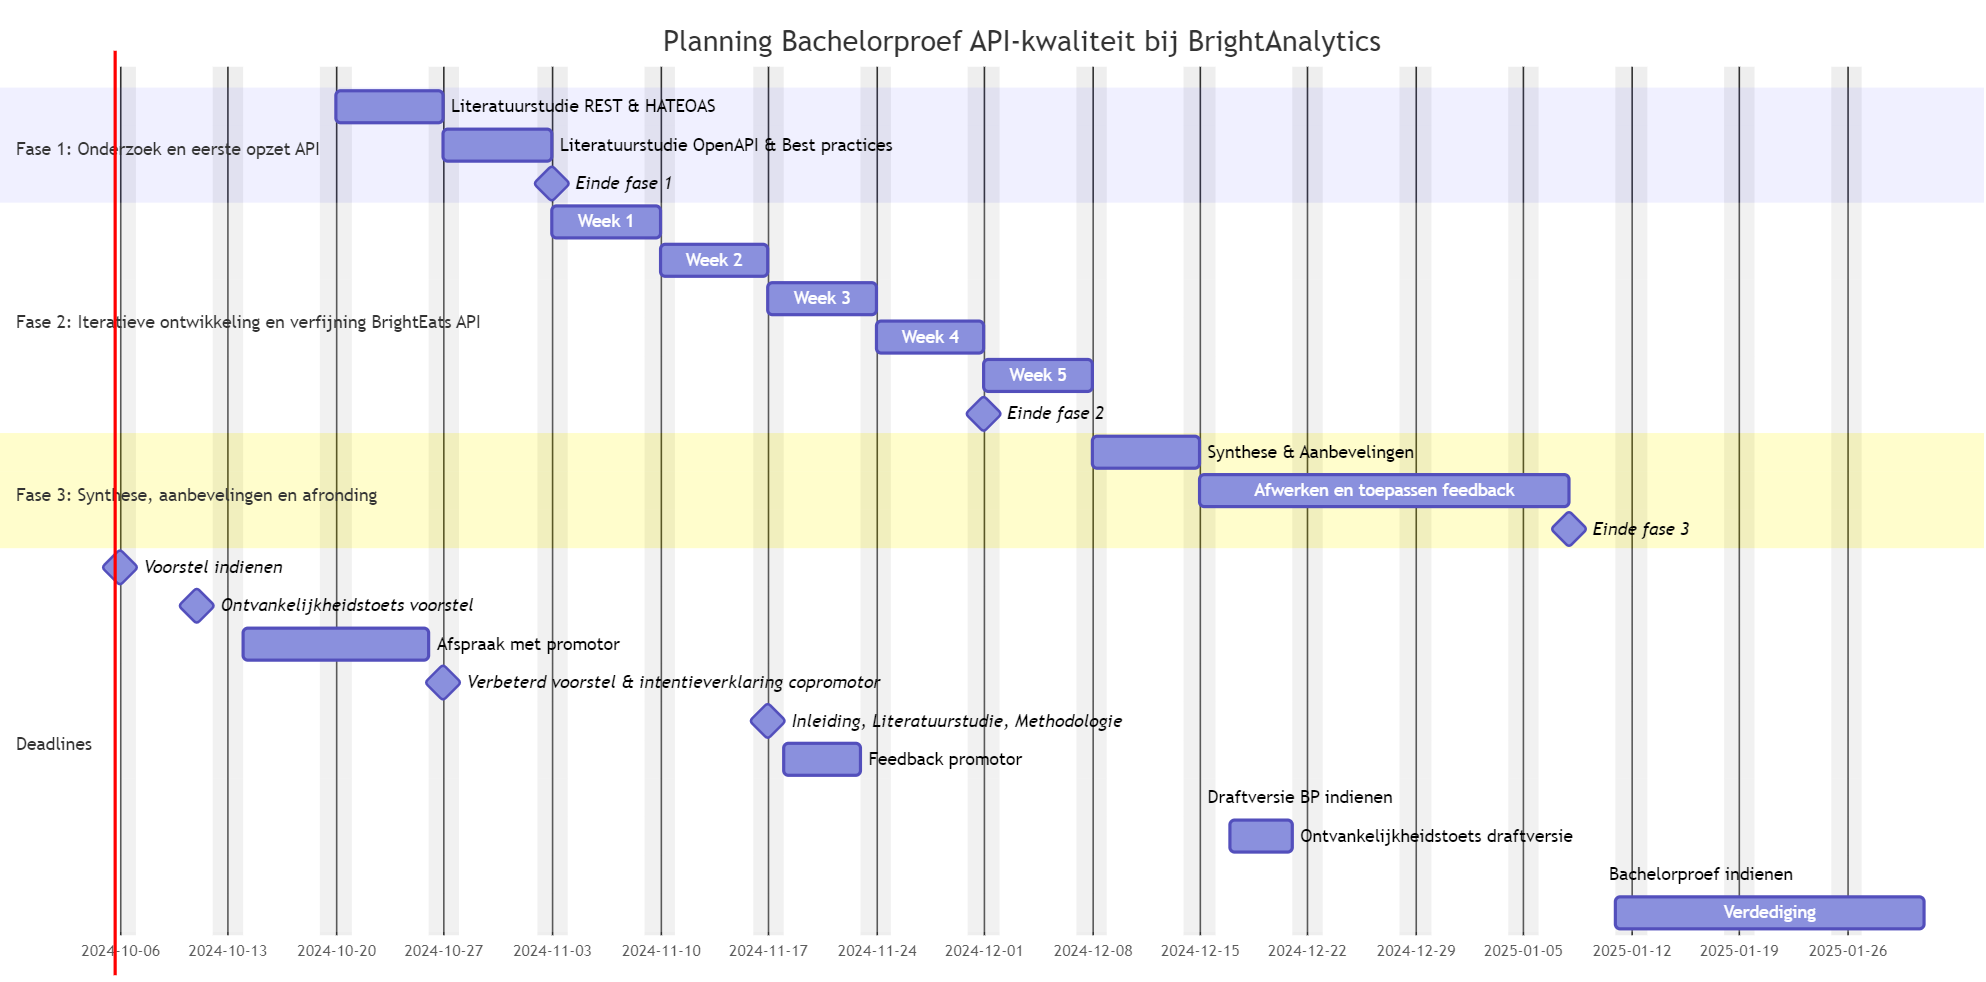
\includegraphics[width=\textwidth, keepaspectratio]{gantt-chart/gantt-chart.png}
  \caption{Gantt chart van de planning van de bachelorproef}
  \label{fig:gantt-chart}
\end{figure}


%%---------- Andere bijlagen --------------------------------------------------
% TODO: Voeg hier eventuele andere bijlagen toe. Bv. als je deze BP voor de
% tweede keer indient, een overzicht van de verbeteringen t.o.v. het origineel.
%\input{...}

%%---------- Backmatter, referentielijst ---------------------------------------

\backmatter{}

\setlength\bibitemsep{2pt} %% Add Some space between the bibliograpy entries
\printbibliography[heading=bibintoc]

\end{document}
